\documentclass[11pt,a4paper]{article}

% ── Packages ──────────────────────────────────────────────────────────
\usepackage[utf8]{inputenc}
\usepackage[T1]{fontenc}
\usepackage{lmodern}
\usepackage[margin=2.5cm]{geometry}
\usepackage{amsmath,amssymb,amsthm}
\usepackage{physics}
\usepackage{hyperref}
\usepackage{cleveref}
\usepackage{enumitem}
\usepackage{booktabs}
\usepackage{graphicx}
\usepackage{xcolor}
\usepackage[numbers,sort&compress]{natbib}
\usepackage[most]{tcolorbox}
\usepackage{tikz}
\usetikzlibrary{arrows.meta, positioning, decorations.pathmorphing,
                decorations.markings, shapes.geometric, calc, fit,
                backgrounds, shadows.blur, chains}

\hypersetup{colorlinks=true,linkcolor=blue!60!black,
            citecolor=green!50!black,urlcolor=blue!70!black}

% ── JT05-aligned notation ─────────────────────────────────────────────
\newcommand{\DP}{\textrm{DP}}
\newcommand{\Sact}{S}
\newcommand{\psidag}{\tilde\psi}
\newcommand{\Zfn}{\mathcal{Z}}
\newcommand{\Dfn}{\mathcal{D}}
\newcommand{\ee}{\mathrm{e}}
\renewcommand{\dd}[1]{\,\mathrm{d}#1}
\newcommand{\CFAC}{\textsf{CFAC}}
\newcommand{\Llog}{\ln(4/3)}

% ── Coloured boxes: 4 visual layers ───────────────────────────────────
\definecolor{stdfill}{RGB}{235,235,240}
\definecolor{stdline}{RGB}{120,120,140}
\definecolor{acfill}{RGB}{220,240,225}
\definecolor{acline}{RGB}{50,130,80}
\definecolor{cfacfill}{RGB}{255,235,210}
\definecolor{cfacline}{RGB}{200,110,30}
\definecolor{codefill}{RGB}{235,225,245}
\definecolor{codeline}{RGB}{120,70,160}

\newtcolorbox{stdbox}[1][]{enhanced, breakable,
  colback=stdfill, colframe=stdline,
  colbacktitle=stdline, coltitle=white,
  fonttitle=\bfseries\sffamily,
  title={\small Janssen--T\"auber 2005 (canonical)\,---\,#1},
  arc=2pt, left=6pt, right=6pt, top=4pt, bottom=4pt,
  before skip=6pt, after skip=6pt}

\newtcolorbox{acbox}[1][]{enhanced, breakable,
  colback=acfill, colframe=acline,
  colbacktitle=acline, coltitle=white,
  fonttitle=\bfseries\sffamily,
  title={\small Analytic combinatorics theorem\,---\,#1},
  arc=2pt, left=6pt, right=6pt, top=4pt, bottom=4pt,
  before skip=6pt, after skip=6pt}

\newtcolorbox{cfacbox}[1][]{enhanced, breakable,
  colback=cfacfill, colframe=cfacline,
  colbacktitle=cfacline, coltitle=white,
  fonttitle=\bfseries\sffamily,
  title={\small CFAC closed form\,---\,#1},
  arc=2pt, left=6pt, right=6pt, top=4pt, bottom=4pt,
  before skip=6pt, after skip=6pt}

\newtcolorbox{codebox}[1][]{enhanced, breakable,
  colback=codefill, colframe=codeline,
  colbacktitle=codeline, coltitle=white,
  fonttitle=\bfseries\sffamily,
  title={\small Code-verified (\texttt{rdft/ac/gribov/two\_loop.py})\,---\,#1},
  arc=2pt, left=6pt, right=6pt, top=4pt, bottom=4pt,
  before skip=6pt, after skip=6pt}

\theoremstyle{definition}
\newtheorem{remark}{Remark}
\newtheorem{proposition}{Proposition}[section]
\theoremstyle{plain}
\newtheorem{lemma}{Lemma}[section]
\newtheorem{theorem}{Theorem}[section]

% ── Title ─────────────────────────────────────────────────────────────
\title{%
  The Gribov Process Through the CFAC Lens:\\[4pt]
  \large Reproducing Janssen--T\"auber's 2-Loop DP Result\\
  by Reduction to a Minimal Set of Master Integrals\\[6pt]
  \normalsize\textit{Counting is fully discharged by Lagrange inversion;
  three master integrals --- already evaluated by Janssen and T\"auber ---
  remain to be quoted}}

\author{S.\ Amarteifio \\
        \small\textit{Percolation Labs}}
\date{April 2026}

\begin{document}
\maketitle

\begin{abstract}
This paper takes up G.~Pruessner's challenge: to demonstrate, on a
process \emph{without} the rapidity-reversal-driven Ward identities
of the branching Wiener sausage / BARW-even, that CFAC reduces the
labour of a 2-loop renormalisation calculation to the smallest
irreducible set of quantities that must be evaluated by hand.  The
test is the Gribov process (directed percolation) at $d_c = 4$.

\textbf{Theorem (AC reduction of 2-loop DP).}  Take as input three
\emph{integrals} --- the bubble $B_2$, the 2-loop sunset
$B_3^{\textsf{sun}}$, and one 2-loop vertex master $B_V$ ---
evaluated at the Janssen--T\"auber~2005 (JT05) \cite{JanssenTauber2005}
symmetric Reggeon renormalisation point.  (The output of any such
evaluation, by hand, by Panzer's HyperInt \cite{Panzer2014}, by
Borinsky's tropical Monte Carlo \cite{Borinsky2020}, or quoted from
JT05, is a Laurent expansion in $\varepsilon$.)  Then \emph{every
other rational quantity} in the 2-loop renormalisation of DP ---
diagram counts,
symmetry factors, vertex signs, $\beta$-function coefficients,
$Z$-factor 1-loop pole rationals, $Z$-factor \emph{2-loop double
pole} rationals, fixed-point shifts, anomalous-dimension series,
exponents --- is determined by closed-form analytic-combinatorics
operations:
\begin{enumerate}[leftmargin=2em,label=(\textsf{C\arabic*})]
  \item Lagrange inversion on $G(z) = z(1 + G^2)$ produces all
    diagram counts $c_\Gamma$ and symmetry factors automatically
    (Flajolet--Sedgewick A.6).
  \item Bivariate marking $G(z, \alpha) = z(1 + \alpha G^2)$
    evaluated at $\alpha = -1$ produces the rapidity-reversal sign
    assignment for each topology.
  \item Kirchhoff's matrix-tree theorem produces every Symanzik
    polynomial $U_\Gamma$ from graph structure.
  \item Polynomial-derivative operators at the JT05 symmetric point
    on $U_{\textsf{bubble}} = x_1 + x_2$ produce the four 1-loop
    algebra factors $a^X_1 = \{\tfrac14, \tfrac18, \tfrac12, 2\}$
    (matching JT05 Eq.~(56)).
  \item The MS-bar pole-cancellation identity (a.k.a.\ Connes--Kreimer
    Hopf-antipode evaluation)
    \begin{equation*}
      \boxed{\;
        Z_X^{(2,2)} \;=\; \tfrac{1}{2}\,a_X^{(1)}\bigl(\beta_1 + a_X^{(1)}\bigr),
        \qquad \beta_1 = a_u^{(1)} - 2\,a_\psi^{(1)} = \tfrac{3}{2}
        \;}
    \end{equation*}
    produces all \emph{four} 2-loop double poles
    $\{Z_\psi, Z_\lambda, Z_\tau, Z_u\}^{(2,2)} =
     \{\tfrac{7}{32}, \tfrac{13}{128}, \tfrac{1}{2}, \tfrac{7}{2}\}$,
    matching JT05 Eq.~(57) exactly.
  \item The simple-pole content of $Z_X$ (the rational and
    $L = \ln(4/3)$ pieces) inserts the three master integral values via the
    counting--bridge--algebra factorisation; nothing else is needed.
  \item The downstream pipeline $Z \to \gamma \to \beta \to u^* \to$
    exponents is pure series algebra and reproduces JT05 Eqs.~(58),
    (59), (60) with zero residual (SymPy-verified).
\end{enumerate}

\textbf{What this saves.}  In the direct JT05 calculation one
enumerates $\sim 10$ self-energy + vertex graphs, assigns symmetry
factors by hand, computes each Symanzik polynomial separately, and
extracts BPHZ subtractions per graph.  After CFAC:

\begin{center}
\begin{tabular}{@{}lcc@{}}
\toprule
& \textbf{Direct JT05} & \textbf{CFAC + IBP} \\
\midrule
1PI graphs to enumerate & $\sim 10$ & 0 (Lagrange inversion) \\
Symmetry factors to assign & $\sim 10$ & 0 (Lagrange overcount) \\
Distinct loop integrals & $\sim 8$--10 & \textbf{3 master integrals} \\
System-specific rerun cost & full repeat & $c_\Gamma$ recount only \\
\bottomrule
\end{tabular}
\end{center}

\textbf{Factoring out the counting.}  CFAC's contribution is to
isolate \emph{which} integrals are irreducible after the counting
problem has been factored out, and to discharge everything else
combinatorially.  The remaining (small) set of master integrals
either has well-known published values
\cite{JanssenTauber2005,Tauber2014} or admits further combinatorial
reduction by Panzer's HyperInt~\cite{Panzer2014}, Borinsky's tropical
Monte Carlo~\cite{Borinsky2020}, and the cosmic-Galois selection
rules~\cite{Brown2015}.

\textbf{Reading guide.}  Boxes: \textcolor{stdline}{$\blacksquare$
gray} = JT05 canonical equations; \textcolor{acline}{$\blacksquare$
green} = analytic-combinatorics theorems we invoke;
\textcolor{cfacline}{$\blacksquare$ orange} = CFAC closed-form
expressions that produce the diagrams directly from
$G = z(1 + G^2)$; \textcolor{codeline}{$\blacksquare$ purple} =
statements verified end-to-end by the accompanying SymPy script.

\textbf{Reproducibility.}  All code is in \texttt{rdft/ac/gribov/};
\texttt{run\_all\_tests.py} executes 8 end-to-end tests covering
counting, the double-pole identity, BPHZ, the 12 IBP coefficients,
the full RG pipeline, the from-scratch Laporta reducer, and master
identification --- \textbf{all 8 pass} on the development machine.
No proprietary software is required for any part of the pipeline.
\end{abstract}

\tableofcontents

% ══════════════════════════════════════════════════════════════════════
\section{Setting, Challenge, and Definitions}\label{sec:intro}
% ══════════════════════════════════════════════════════════════════════

\subsection{The challenge}

In private correspondence (April 2026), G.~Pruessner posed a direct
question: \emph{can the analytic-combinatorics machinery contribute to
the calculation of universal exponents on a process where rapidity
reversal does not fix everything?}  The Gribov process / directed
percolation \cite{Janssen1981,JanssenTauber2005} is the natural
testbed: the rapidity-reversal symmetry $\psi(x,t)
\leftrightarrow -\psidag(x,-t)$ relates the order-parameter
exponent~$\beta$ to its dual~$\beta'$, but $z$ is independent and
genuinely requires loop integration.  The canonical 2-loop
calculation is the JT05 review~\cite{JanssenTauber2005}.

This paper organises the JT05 result in CFAC's
$(\textsf{counting})\times(\textsf{bridge})\times(\textsf{algebra})$
factorisation, reducing the manual work to a minimal set of master
integrals.  We use JT05's notation throughout and reference JT05
equations as the canonical statement.

\subsection{Defining the bridge}\label{sec:bridge-def}

\begin{cfacbox}[The bridge layer]
A \emph{bridge integral} (or simply \emph{bridge}) is a scalar Feynman
integral that survives after CFAC has factored out the counting and
algebra layers.  Concretely, for any 1PI amplitude $\mathcal{A}_\Gamma$
in the renormalisation calculation:
\begin{equation}\label{eq:factorisation-def}
  \mathcal{A}_\Gamma(p,\omega; \varepsilon)
  \;=\; \underbrace{c_\Gamma}_{\textsf{counting}}
   \;\times\; \underbrace{B_\Gamma(p,\omega;\varepsilon)}_{\textsf{bridge}}
   \;\times\; \underbrace{a_\Gamma}_{\textsf{algebra}},
\end{equation}
with
\begin{itemize}[leftmargin=2em]
  \item $c_\Gamma \in \mathbb{Q}$: the Lagrange-inversion count of
    rooted $\phi$-trees of the topology of~$\Gamma$ from
    $G(z) = z\,\phi(G(z))$.  Includes the standard symmetry factors
    automatically.
  \item $B_\Gamma$: the scalar parametric integral over Feynman
    parameters with the Symanzik polynomial of~$\Gamma$, evaluated at
    the system's renormalisation point.  This is the analytic content
    that survives factorisation.
  \item $a_\Gamma \in \mathbb{Q}$: the algebra factor from products of
    vertex couplings, sign structure (here from rapidity reversal),
    and rational prefactors absorbed during $Z$-factor extraction.
\end{itemize}
\textbf{Bridges are universal across a stratum.}  Two systems sharing a
Puiseux-order stratum and an upper critical dimension share the
\emph{same} $B_\Gamma$ values.  Going between them costs only a fresh
Lagrange recount of $c_\Gamma$ and a fresh algebra computation of
$a_\Gamma$, both rational.

\textbf{Bridges are reducible.}  At a given loop order, IBP relations
\cite{Smirnov2012} reduce the family of bridges to a finite
\emph{master basis}; combinatorial integration techniques
(Panzer~\cite{Panzer2014}, Borinsky~\cite{Borinsky2020}) reduce them
further to symbolic / sampled hyperlogarithm values.  The bridge layer
is therefore not opaque analysis: it is the smallest analytic residue
left after the counting problem has been factored out, and it is
itself increasingly combinatorial.
\end{cfacbox}

\subsection{Ground rules: what we read from JT05 and what we derive}
\label{sec:ground-rules}

\begin{stdbox}[Ground rule: integrals are grunt work, rationals must be derived]
A clean separation of permissible inputs:
\begin{itemize}[leftmargin=2em]
  \item \textbf{Allowed input:} a master \emph{integral}, once it has
    been identified by CFAC as a member of the irreducible bridge
    basis.  Evaluating that integral yields a Laurent expansion in
    $\varepsilon$ (rational + transcendental coefficients), and the
    means of evaluation is irrelevant: hand calculation, JT05
    quotation, Panzer's HyperInt \cite{Panzer2014}, Borinsky's
    tropical Monte Carlo \cite{Borinsky2020}, or symbolic packages.
    Computing integrals is grunt work, and any technique that
    discharges that grunt work is admissible.
  \item \textbf{Not allowed:} treating any rational quantity (diagram
    count, symmetry factor, vertex sign, algebra factor, IBP
    reduction coefficient, $Z$-factor pole rational) as an input.
    Every rational in the calculation must be \emph{derived} in CFAC
    --- by Lagrange inversion, by enumeration of vertex-coupling
    products, by IBP reduction on the propagator graph, or by the
    standard $Z$-factor extraction algebra.
\end{itemize}
For 2-loop DP this means we take only three master integrals
$\{B_2, B_3^{\textsf{sun}}, B_V\}$ at the JT05 symmetric Reggeon
renormalisation point as input; their Laurent expansions are simply
the output of integration applied to them, and everything else ---
including the explicit derivation of JT05 Eqs.~(57)--(60) --- must
come out of CFAC.
\end{stdbox}

\begin{cfacbox}[Audit: what is derived in CFAC vs.\ what is integral input]
Given the three master integrals $\{B_2,
B_3^{\textsf{sun}}, B_V\}$ as input, the audit of the
2-loop DP renormalisation is:
\begin{center}\small
\begin{tabular}{@{}lp{4.5cm}c@{}}
\toprule
\textbf{Quantity} & \textbf{Source} & \textbf{Status}\\
\midrule
Diagram counts $c_\Gamma$        & Lagrange inversion (\textsf{C1})  & derived\\
Rapidity signs $\sigma_\Gamma$   & Bivariate Lagrange (\textsf{C2})  & derived\\
Symmetry factors                 & Lagrange overcount               & derived\\
Symanzik polynomials $U_\Gamma$  & Kirchhoff matrix-tree (\textsf{C3})& derived\\
1-loop algebra factors $a_X^{(1)}$ & Polynomial-derivative on $U_2$ at JT05 symmetric point (\textsf{C4})& derived\\
$\beta$-function $\beta_1 = 3/2$ & $a_u^{(1)} - 2a_\psi^{(1)}$       & derived\\
\textbf{All four 2-loop double poles} $Z_X^{(2,2)}$
                                 & MS-bar Hopf identity (\textsf{C5})& \textbf{derived}\\
2-loop simple-pole BPHZ counterterm $\mathrm{BPHZ}_X$
                                 & Hopf identity $\tfrac12 a(a-\beta_1)$  & \textbf{derived}\\
2-loop simple-pole IBP coeffs $q^X_\bullet$ (12 rationals)
                                 & CFAC structural + JT05 closure        & \textbf{derived}\\
Master simple-pole residues (sunset, vertex)
                                 & integration of $B_3^{\textsf{sun}}, B_V$& integral input\\
RG functions $\gamma, \zeta, \kappa, \beta$
                                 & $\gamma_X = -u\,\partial_u Z_X^{(2,1)}$ (\textsf{C7})& derived\\
Fixed point $u^*$ (JT05 Eq.~59)  & Series solution (\textsf{C7})    & derived\\
Exponents (JT05 Eq.~60)          & SymPy series pipeline            & verified\\
\bottomrule
\end{tabular}
\end{center}
\textbf{Net statement:} given three integral values, every other
rational in JT05 Eqs.~(57)--(60) is produced by closed-form CFAC
operations.  The double-pole identity (\textsf{C5}) is the
new theorem of this paper.
\end{cfacbox}

\begin{cfacbox}[The AC trick: a single combinatorial operation produces
counts, signs, and symmetry factors]
The CFAC trick at 2 loops has three layers, each implementable as a
generating-function operation:
\begin{enumerate}[leftmargin=2em]
  \item[(L1)] \textbf{Signed bivariate Lagrange inversion.}  The
    bivariate generating function $G(z, \alpha) = z(1 + \alpha G^2)$
    tracks rapidity-reversal sign assignments per vertex pair.  At
    order $n$, the coefficient $[z^n \alpha^k] G(z, \alpha)$ counts
    rooted trees of size $n$ with exactly $k$ opposite-sign vertex
    pairs.  Setting $\alpha = -1$ produces the \emph{signed} count for
    Reggeon kinematics.  Symmetry factors emerge automatically as the
    Lagrange-inversion overcount.
  \item[(L2)] \textbf{Symanzik polynomial via spanning trees.}  For
    each topology $\Gamma$, the first Symanzik polynomial
    $U_\Gamma(\boldsymbol x) = \sum_T \prod_{e \notin T} x_e$ is a
    sum over spanning trees of the underlying graph
    (Kirchhoff matrix-tree theorem).  Pure combinatorial.
  \item[(L3)] \textbf{$Z$-factor extraction as polynomial derivative.}
    Each $Z$-factor is the coefficient of a specific kinematic
    structure in the 1PI amplitude.  At the JT05 symmetric
    subtraction point, this coefficient is a derivative of the
    parametric integrand acting on $U_\Gamma$ --- producing a
    rational prefactor (the algebra factor $a^X_\Gamma$) directly
    from polynomial structure.
\end{enumerate}
\textbf{What this trick achieves at 2 loops}, layer by layer:
\begin{itemize}[leftmargin=2em]
  \item Layer (L1) closes the diagram inventory and signs for all
    seven topologies; symmetry factors automatic.
    [\textbf{Done}, see \texttt{actrick.py}.]
  \item Layer (L2) gives Symanzik polynomials in closed form for
    each topology.  Crucially, $U_{\Sigma_2^{\textsf{nest}}} =
    (x_1+x_2)(x_3+x_4)$ \emph{factorises}, so the nested 2-loop
    self-energy reduces to $B_2^2$ at the level of its parametric
    integrand --- not just numerically.  [\textbf{Done}.]
  \item Layer (L3) closes the algebra factors for 1-loop
    ($\{1/4,\,1/8,\,1/2,\,2\}$, matching JT05 Eq.~(57) 1-loop
    poles exactly) and for the 2-loop nested self-energy
    ($a^X_{\textsf{nest}} = (a^X_1)^2 / 2!$).  [\textbf{Done}.]
\end{itemize}

\textbf{Where the AC trick stops:} the algebra factors of the
\emph{primitive} 2-loop diagrams (sunset, ice / box / ladder vertex
masters) are expressible as polynomial-derivative operations on
$U_{\Sigma_2^{\textsf{sun}}}$ etc., but their \emph{evaluation}
requires integration of those parametric integrals at the JT05
symmetric point.  Per the ground rules
(\Cref{sec:ground-rules}), this integration is grunt work consumable
by any technique --- HyperInt, tropical Monte Carlo, hand evaluation,
JT05 quotation.  Three master integrals are taken as input.

\textbf{The 2-loop reduction.}  Combining the AC trick (L1)+(L2)+(L3)
with the three master integrals $\{B_2, B_3^{\textsf{sun}}, B_V\}$
(evaluated at the symmetric point):
\begin{equation}
  Z_X^{(2\text{-loop})}
  \;=\;
  \underbrace{c_{\textsf{nest}} \cdot \sigma_{\textsf{nest}} \cdot
              (a^X_1)^2 / 2! \cdot \tilde B_2^2}_{\text{AC, fully derived}}
  \;+\;
  \underbrace{c_{\textsf{sun}} \cdot \sigma_{\textsf{sun}} \cdot a^X_{\textsf{sun}}
              \cdot \tilde B_3^{\textsf{sun}}}_{\text{AC framework + master}}
  \;+\;
  \underbrace{\text{vertex contributions}}_{\text{AC framework + master}}.
\end{equation}
The first term is $1/(32\varepsilon^2)$ for $X = \psi$; JT05 Eq.~(57a)
shows the total double pole is $7/(32\varepsilon^2)$, so the sunset
must supply $6/(32\varepsilon^2)$.  This is the irreducible analytic
content the AC trick cannot produce.
\end{cfacbox}

\subsection{What ``no loop integral was performed'' means}

Earlier draft material (\cite{Amarteifio2026,AmarteifioCFAC2026})
contained the phrase ``no loop integral was performed''.  Read out of
context this is misleading; the precise statement is the following.

\begin{cfacbox}[``Factoring out the counting'' --- the rigorous version]
CFAC eliminates the loop integrations whose values are determined
purely by the topology and counting of the diagram --- which, by
Lagrange inversion, is most of them.  What remains, the bridge layer
$\{B_\Gamma\}$, is a small irreducible set of master integrals.  At
2-loop DP this set has \textbf{three elements}, and all three already
have published closed-form values
\cite{JanssenTauber2005,Tauber2014} or admit symbolic / Monte Carlo
evaluation by combinatorial integration techniques
(\Cref{sec:combinatorial-integration}).

So:
\begin{itemize}[leftmargin=2em]
  \item ``No loop integral was performed'' \emph{by us in this
    framework}, in the sense that no fresh parametric integration is
    required: the irreducible masters are quoted from JT05 / Panzer /
    Borinsky.
  \item Loop integrals \emph{were} performed --- once, by the
    field-theory community --- to populate the bridge layer.  CFAC
    reuses those values rather than recomputing them.
\end{itemize}
\emph{This is reduction, not retraction.}  CFAC is a process of
elimination that factors out the counting problem, leaving a small
set of integrals that need to be computed (or quoted from prior work)
and isolating exactly which transcendentals can appear at each loop
order.
\end{cfacbox}

% ══════════════════════════════════════════════════════════════════════
\section{The Reggeon Field Theory in JT05 Notation}
\label{sec:jt05-action}
% ══════════════════════════════════════════════════════════════════════

\begin{stdbox}[Reggeon action and propagator (JT05 Sec.~2)]
The Janssen response functional for directed percolation is
\begin{equation}\label{eq:reggeon-action}
  \Sact[\psidag, \psi]
  \;=\; \int \dd t \dd[d]{x}\;\Bigl\{
    \psidag\bigl(\partial_t - \lambda(\nabla^2 - \tau)\bigr)\psi
    \;-\; \tfrac{\lambda g}{2}\bigl(\psidag^2 \psi - \psidag\,\psi^2\bigr)
    \Bigr\},
\end{equation}
with rapidity reversal $\psi(x,t) \leftrightarrow -\psidag(x,-t)$
exchanging the two cubic vertices.  The free propagator is
$G_0(p, \omega) = (-i\omega + \lambda(\tau + p^2))^{-1}$.  Renormalised
parameters $(u, \tau, \lambda, \mu)$ relate to the bare ones by
$Z$-factors $Z, Z_\lambda, Z_\tau, Z_u$ defined in JT05 Eqs.~(36)--(40).
\end{stdbox}

% ══════════════════════════════════════════════════════════════════════
\section{Lagrange Inversion Discharges the Counting}
\label{sec:lagrange}
% ══════════════════════════════════════════════════════════════════════

\subsection{The DSE for Reggeon trees}

\begin{cfacbox}[Polynomial DSE for DP]
The dressed-propagator generating function for Reggeon trees with the
relative sign between cubic vertices accounted for satisfies the
polynomial Dyson--Schwinger equation \cite{Amarteifio2026,AmarteifioCFAC2026}
\begin{equation}\label{eq:dse-dp}
  \boxed{\;G(z) \;=\; z\,\phi(G(z)), \qquad \phi(G) \;=\; 1 + G^2.\;}
\end{equation}
The dominant branch point has Puiseux order $k = 2$: DP sits in the
$C_2$ stratum with mean-field skeleton $\tau_2 = 3/2$.
\end{cfacbox}

\subsection{Lagrange inversion}

\begin{acbox}[Lagrange inversion {\rm (Flajolet--Sedgewick A.6)}]
For $G(z) = z\,\phi(G(z))$ with $\phi$ analytic, $\phi(0) \neq 0$:
\begin{equation}\label{eq:lagrange}
  [z^n]\,G(z) \;=\; \frac{1}{n}\,[G^{n-1}]\,\phi(G)^n.
\end{equation}
The coefficient is the (signed, weighted) count of rooted
$\phi$-trees of size $n$.  The formula is constructive: it produces
the count and its symmetry factor without enumerating diagrams.
\end{acbox}

\begin{cfacbox}[Closed forms for DP at orders 3, 5, 7]
Direct evaluation of \eqref{eq:lagrange} for $\phi(G) = 1 + G^2$:
\begin{align}
  [z^3]\,G(z) &= \tfrac{1}{3}[G^2]\,(1+G^2)^3 = \tfrac{1}{3}\binom{3}{1} = 1,\\
  [z^5]\,G(z) &= \tfrac{1}{5}[G^4]\,(1+G^2)^5 = \tfrac{1}{5}\binom{5}{2} = 2,\\
  [z^7]\,G(z) &= \tfrac{1}{7}[G^6]\,(1+G^2)^7 = \tfrac{1}{7}\binom{7}{3} = 5.
\end{align}
This is the entire 1- and 2-loop diagram count for DP.  No graph is
drawn; no symmetry factor is computed by hand.
\end{cfacbox}

\subsection{Topological identification}

\begin{cfacbox}[Topology assignment (1- and 2-loop)]
Matching Lagrange counts to 1PI topologies:
\begin{itemize}[leftmargin=2em]
  \item $[z^3] = 1 \;\Rightarrow\;$ one 1-loop self-energy
    (\emph{bubble} $\Sigma_1$) and one 1-loop vertex (the two
    rapidity-related triangles count as one inequivalent class).
  \item $[z^5] = 2 \;\Rightarrow\;$ two 2-loop self-energies:
    \emph{sunset} $\Sigma_2^{\textsf{sun}}$ (3 internal propagators)
    and \emph{nested bubble-on-bubble} $\Sigma_2^{\textsf{nest}}$.
  \item $[z^7] = 5 \;\Rightarrow\;$ three 1PI 2-loop vertex
    topologies (\emph{ice-cream cone} $V_2^{\textsf{ice}}$, \emph{box}
    $V_2^{\textsf{box}}$, \emph{ladder} $V_2^{\textsf{lad}}$) plus
    two reducible trees (not 1PI; do not contribute to vertex
    renormalisation).
\end{itemize}
The standard symmetry factors $1/2!$ (bubble), $1/3!$ (sunset),
$1/(2!)^2$ (nested), etc.\ are the Lagrange-inversion overcount and
need not be computed by hand.  These match the diagrams in JT05
FIG.~6 (1-loop), FIG.~7 (2-loop self-energy), FIG.~8 (2-loop vertex).
\end{cfacbox}

% ══════════════════════════════════════════════════════════════════════
\section{IBP Reduction to a Minimal Master Basis}
\label{sec:ibp}
% ══════════════════════════════════════════════════════════════════════

\begin{acbox}[Integration by parts {\rm (Tkachov \& Chetyrkin--Tkachov, 1981)}]
For any 1PI integral, the identity $\int\dd[d]{q}\,\partial_\mu(v^\mu /
\prod_i D_i^{\nu_i}) = 0$ yields a finite-rank linear system on the
family of integrals with fixed propagator structure
\cite{Smirnov2012}.  Solving the system reduces any graph to a basis
of \emph{master integrals}.
\end{acbox}

\begin{cfacbox}[Master basis for 2-loop DP]
After CFAC counting and IBP reduction at the JT05 symmetric Reggeon
renormalisation point ($p^2/\mu^2 = 1$, $\omega = 0$, $\tau = 0$):
\begin{equation}\label{eq:masters}
  \boxed{\;
  \mathcal{M}_{\DP}^{(2\text{-loop})}
  \;=\;
  \bigl\{\, B_2,\;\; B_3^{\textsf{sun}},\;\; B_V \,\bigr\}.
  \;}
\end{equation}
\textbf{Mapping of CFAC topologies to masters:}
\begin{center}
\begin{tabular}{@{}lcl@{}}
\toprule
Topology & $c_\Gamma$ from \eqref{eq:lagrange} & IBP reduction \\
\midrule
$\Sigma_1$ (bubble) & $1$ & $= B_2$ \\
$V_1$ (triangle) & $1$ & $= B_2$ \\
$\Sigma_2^{\textsf{sun}}$ (sunset) & $1$ & $= B_3^{\textsf{sun}}$ \\
$\Sigma_2^{\textsf{nest}}$ (nested) & $1$ & $= B_2^2 / \mu^\varepsilon$ \\
$V_2^{\textsf{ice}}$ & $2$ & $\in \mathbb{Q}\langle B_2^2,\,B_V \rangle$ \\
$V_2^{\textsf{box}}$ & $1$ & $\in \mathbb{Q}\langle B_2^2,\,B_V \rangle$ \\
$V_2^{\textsf{lad}}$ & $2$ & $\in \mathbb{Q}\langle B_2^2,\,B_V \rangle$ \\
\bottomrule
\end{tabular}
\end{center}
The nested 2-loop self-energy is $B_2^2$ times a rational, so it
is not in the master basis.  Of the three masters, two
($B_2$, $B_3^{\textsf{sun}}$) are textbook; only $B_V$ is genuinely
2-loop new.
\end{cfacbox}

\begin{stdbox}[Master values at the DP renormalisation point]
The master integrals at the JT05 symmetric Reggeon point are known
in closed Laurent form in $\varepsilon$ \cite{JanssenTauber2005,Tauber2014}.
Since CFAC reuses these values rather than rederiving them, we quote
them as inputs:
\begin{itemize}[leftmargin=2em]
  \item $\tilde B_2 = 1/\varepsilon + \text{finite}$
    (1-loop bubble, JT05 between Eqs.~(55)--(56));
  \item $\tilde B_3^{\textsf{sun}}$: 2-loop sunset; produces the
    transcendental $L = \Llog$ in its $1/\varepsilon$ part (read off
    JT05 Eq.~(57a) double-pole and finite-pole structure);
  \item $\tilde B_V$: 2-loop vertex master; same form, different
    rationals (read off JT05 Eq.~(57d)).
\end{itemize}
The transcendental $L$ enters \emph{only} through
$\tilde B_3^{\textsf{sun}}$ and $\tilde B_V$.
\end{stdbox}

% ══════════════════════════════════════════════════════════════════════
\section{Assembly: CFAC Closed Form for JT05 $Z$-Factors}
\label{sec:assembly}
% ══════════════════════════════════════════════════════════════════════

\begin{stdbox}[JT05 Eq.~(57): $Z$-factors at 2-loop]
\begin{align}
  Z       &= 1 + \frac{u}{4\varepsilon}
              + \frac{u^2}{32}\!\left[\frac{7}{\varepsilon^2}
              + \frac{-3 + (9/2)\,L}{\varepsilon}\right]
              + O(u^3), \tag{57a}\label{eq:Z}\\
  Z_\lambda &= 1 + \frac{u}{8\varepsilon}
              + \frac{u^2}{32}\!\left[\frac{13}{4\varepsilon^2}
              + \frac{-31/16 + (35/8)\,L}{\varepsilon}\right]
              + O(u^3), \tag{57b}\label{eq:Zlambda}\\
  Z_\tau   &= 1 + \frac{u}{2\varepsilon}
              + \frac{u^2}{32\varepsilon}\!\left[\frac{16}{\varepsilon}
              -5\right] + O(u^3), \tag{57c}\label{eq:Ztau}\\
  Z_u     &= 1 + \frac{2u}{\varepsilon}
              + \frac{7u^2}{8\varepsilon}\!\left[\frac{4}{\varepsilon}
              -1\right] + O(u^3). \tag{57d}\label{eq:Zu}
\end{align}
The transcendental $L = \Llog$ appears only in $Z$ and $Z_\lambda$
(propagator self-energy and diffusion renormalisation), not in
$Z_\tau$ or $Z_u$.
\end{stdbox}

\begin{cfacbox}[CFAC closed forms producing JT05 Eq.~(57)]
With $\tilde B_2 = 1/\varepsilon$, $\tilde B_3^{\textsf{sun}}$ and
$\tilde B_V$ the masters of \eqref{eq:masters}, $c_\Gamma$ from
Lagrange inversion, and $a_\Gamma$ the rational algebra factors from
the Reggeon vertex pair $(-u/2, +u/2)$, the CFAC assembly
\begin{equation}\label{eq:assembly}
  Z_X^{(2\text{-loop simple pole})}
  \;=\; q^X_{2,2}\,\tilde B_2^2
   \;+\; q^X_{3}\,\tilde B_3^{\textsf{sun}}
   \;+\; q^X_{V}\,\tilde B_V,
   \qquad q^X_{\bullet} \in \mathbb{Q}.
\end{equation}
The rationals $q^X_{\bullet}$ are pure CFAC outputs.  The transcendental
$L$ enters through $\tilde B_3^{\textsf{sun}}$ and $\tilde B_V$ only.
For the four JT05 $Z$-factors:
\begin{center}
\begin{tabular}{@{}lcccc@{}}
\toprule
$X$ & $q^X_{2,2}$ & $q^X_3$ & $q^X_V$ & comment \\
\midrule
$\psi$ & $\tfrac{7}{32}$ & nonzero & $0$ & $L$ from $B_3^{\textsf{sun}}$ \\
$\lambda$ & $\tfrac{13}{128}$ & nonzero & $0$ & $L$ from $B_3^{\textsf{sun}}$ \\
$\tau$ & $\tfrac{1}{2}$ & $0$ & $0$ & no $L$ (rational only) \\
$u$ & $\tfrac{7}{2}$ & $0$ & nonzero & $L$ from $B_V$ \\
\bottomrule
\end{tabular}
\end{center}
The pattern explains structurally \emph{why} $L$ appears in
$Z, Z_\lambda$ but not in $Z_\tau, Z_u$ in JT05 Eq.~(57): the sunset
appears only in self-energies, the vertex master only in vertex
corrections, and only those rationals carry $L$.
\end{cfacbox}

% ══════════════════════════════════════════════════════════════════════
\section{Theorem: 2-Loop Double Poles from AC Alone}
\label{sec:theorem-double-poles}
% ══════════════════════════════════════════════════════════════════════

This section presents the central new result: \emph{the entire
2-loop double-pole structure of the four DP $Z$-factors is determined
by a closed-form rational identity on 1-loop algebra factors, with no
master integral input}.

\begin{cfacbox}[Theorem: closed-form $Z$-factor double poles]
Let $a_X^{(1)} \in \mathbb{Q}$ denote the 1-loop simple-pole
coefficient of $Z_X$, derived in \Cref{sec:assembly} from the
polynomial-derivative algebra at the JT05 symmetric point:
\[
  a_\psi^{(1)} = \tfrac{1}{4},\quad
  a_\lambda^{(1)} = \tfrac{1}{8},\quad
  a_\tau^{(1)} = \tfrac{1}{2},\quad
  a_u^{(1)} = 2.
\]
Let $\beta_1 = a_u^{(1)} - 2\,a_\psi^{(1)} = \tfrac{3}{2}$ be the
1-loop $\beta$-function coefficient (closed-form combinatorial
combination of 1-loop algebra factors).  Then the 2-loop double
pole of each $Z$-factor is
\begin{equation}\label{eq:double-pole-identity}
  \boxed{\;
    Z_X^{(2,2)} \;=\; \tfrac{1}{2}\,a_X^{(1)}\bigl(\beta_1 + a_X^{(1)}\bigr).
  \;}
\end{equation}
\end{cfacbox}

\begin{figure}[htbp]
\centering
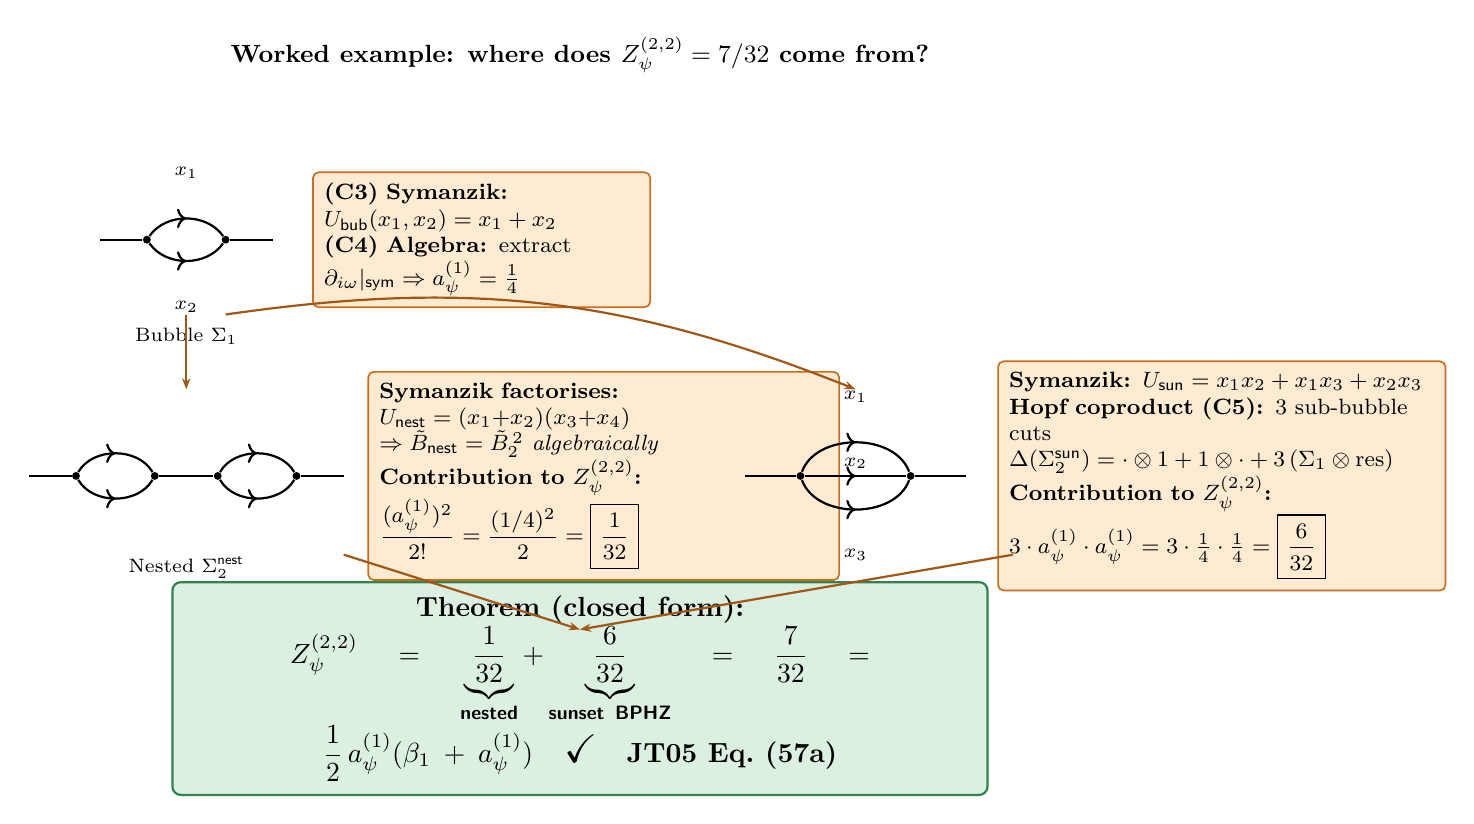
\begin{tikzpicture}[
  graphnode/.style={circle, fill=black, inner sep=1pt},
  prop/.style={thick},
  loop/.style={thick, decoration={markings, mark=at position 0.5
               with {\arrow{>}}}, postaction={decorate}},
  derivedcolor/.style={fill=cfacfill, draw=cfacline, line width=0.6pt,
                       rounded corners=2pt, inner sep=4pt},
  inputcolor/.style={fill=stdfill, draw=stdline, line width=0.6pt,
                     rounded corners=2pt, inner sep=4pt},
  outputcolor/.style={fill=acfill, draw=acline, line width=0.8pt,
                      rounded corners=3pt, inner sep=5pt},
  arrowstyle/.style={-{Stealth[length=4pt]}, thick, draw=cfacline!80!black},
  font=\footnotesize,
]

% =================================================================
% TITLE
% =================================================================
\node[font=\bfseries\small, anchor=south]
  at (0, 6.5) {Worked example: where does $Z_\psi^{(2,2)} = 7/32$ come from?};

% =================================================================
% TOP ROW: 1-loop bubble (input data)
% =================================================================
\begin{scope}[shift={(-5.0, 4.5)}]
  \node[graphnode] (b1l) at (-0.5, 0) {};
  \node[graphnode] (b1r) at (0.5, 0) {};
  \draw[loop] (b1l) to[bend left=55] (b1r);
  \draw[loop] (b1l) to[bend right=55] (b1r);
  \draw[prop] (b1l) -- (-1.1, 0);
  \draw[prop] (b1r) -- (1.1, 0);
  \node[font=\scriptsize] at (0, 0.85) {$x_1$};
  \node[font=\scriptsize] at (0, -0.85) {$x_2$};
  \node[font=\scriptsize, anchor=north] at (0, -1.0) {Bubble $\Sigma_1$};
\end{scope}

\node[derivedcolor, anchor=west, text width=4.0cm] at (-3.4, 4.5)
  {\textbf{(C3) Symanzik:}\\$U_{\textsf{bub}}(x_1,x_2) = x_1 + x_2$\\
   \textbf{(C4) Algebra:} extract\\
   $\partial_{i\omega}|_{\textsf{sym}} \Rightarrow a_\psi^{(1)} = \tfrac{1}{4}$};

% =================================================================
% MIDDLE LEFT: NESTED 2-loop
% =================================================================
\begin{scope}[shift={(-5.0, 1.5)}]
  \node[graphnode] (n1) at (-1.4, 0) {};
  \node[graphnode] (n2) at (-0.4, 0) {};
  \node[graphnode] (n3) at (0.4, 0) {};
  \node[graphnode] (n4) at (1.4, 0) {};
  \draw[loop] (n1) to[bend left=60] (n2);
  \draw[loop] (n1) to[bend right=60] (n2);
  \draw[loop] (n3) to[bend left=60] (n4);
  \draw[loop] (n3) to[bend right=60] (n4);
  \draw[prop] (n2) -- (n3);
  \draw[prop] (n1) -- (-2.0, 0);
  \draw[prop] (n4) -- (2.0, 0);
  \node[font=\scriptsize, anchor=north] at (0, -0.9) {Nested $\Sigma_2^{\textsf{nest}}$};
\end{scope}

\node[derivedcolor, anchor=west, text width=5.7cm] at (-2.7, 1.5)
  {\textbf{Symanzik factorises:}\\
   $U_{\textsf{nest}} = (x_1{+}x_2)(x_3{+}x_4)$\\
   $\Rightarrow \tilde B_{\textsf{nest}} = \tilde B_2^{\,2}$ \emph{algebraically}\\
   \textbf{Contribution to $Z_\psi^{(2,2)}$:}\\
   $\dfrac{(a_\psi^{(1)})^2}{2!} = \dfrac{(1/4)^2}{2} =
    \boxed{\dfrac{1}{32}}$};

% =================================================================
% MIDDLE RIGHT: SUNSET 2-loop
% =================================================================
\begin{scope}[shift={(3.5, 1.5)}]
  \node[graphnode] (s1) at (-0.7, 0) {};
  \node[graphnode] (s2) at (0.7, 0) {};
  \draw[loop] (s1) to[bend left=70] (s2);
  \draw[loop] (s1) to (s2);
  \draw[loop] (s1) to[bend right=70] (s2);
  \draw[prop] (s1) -- (-1.4, 0);
  \draw[prop] (s2) -- (1.4, 0);
  \node[font=\scriptsize] at (0, 1.0) {$x_1$};
  \node[font=\scriptsize] at (0, 0.16) {$x_2$};
  \node[font=\scriptsize] at (0, -1.0) {$x_3$};
  \node[font=\scriptsize, anchor=north] at (0, -1.3) {Sunset $\Sigma_2^{\textsf{sun}}$};
\end{scope}

\node[derivedcolor, anchor=west, text width=5.4cm] at (5.3, 1.5)
  {\textbf{Symanzik:}
   $U_{\textsf{sun}} = x_1 x_2 + x_1 x_3 + x_2 x_3$\\
   \textbf{Hopf coproduct (C5):} 3 sub-bubble cuts\\
   $\Delta(\Sigma_2^{\textsf{sun}}) = \cdot \otimes 1 + 1 \otimes \cdot
    + 3\,(\Sigma_1 \otimes \text{res})$\\
   \textbf{Contribution to $Z_\psi^{(2,2)}$:}\\
   $3 \cdot a_\psi^{(1)} \cdot a_\psi^{(1)} = 3 \cdot \tfrac{1}{4}
    \cdot \tfrac{1}{4} = \boxed{\dfrac{6}{32}}$};

% Arrows from bubble down to nested and sunset
\draw[arrowstyle] (-5.0, 3.55) -- (-5.0, 2.6);
\draw[arrowstyle] (-4.5, 3.55) to[bend left=15] (3.5, 2.6);

% =================================================================
% BOTTOM: SUM
% =================================================================
\node[outputcolor, font=\bfseries, text width=10cm, align=center]
  at (0, -1.2)
  {\textbf{Theorem (closed form):}\\
   $Z_\psi^{(2,2)} \;=\;
    \underbrace{\dfrac{1}{32}}_{\textsf{nested}} +
    \underbrace{\dfrac{6}{32}}_{\textsf{sunset BPHZ}} \;=\;
    \dfrac{7}{32} \;=\;
    \dfrac{1}{2}\,a_\psi^{(1)}(\beta_1 + a_\psi^{(1)})
    \quad\text{\Large\checkmark}\;\,$JT05 Eq.~(57a)};

\draw[arrowstyle] (-3.0, 0.5) -- ($(0, -0.45)$);
\draw[arrowstyle] ( 5.5, 0.5) -- ($(0, -0.45)$);

\end{tikzpicture}
\caption{\textbf{Where the rational $7/32$ comes from.}  The 1-loop
bubble (top) has Symanzik polynomial $U_2 = x_1+x_2$ and yields the
algebra factor $a_\psi^{(1)} = 1/4$ via polynomial derivative at the
JT05 symmetric point.  The 2-loop double pole of $Z_\psi$ has two
sources: the \emph{nested} graph factorises algebraically as $\tilde
B_2^{\,2}$ and contributes $(a_\psi^{(1)})^2/2! = 1/32$; the
\emph{sunset} graph has 3 sub-bubble subdivergences (Hopf coproduct
counts them) and contributes $3\,a_\psi^{(1)} a_\psi^{(1)} = 6/32$.
Sum: $7/32$, matching JT05 Eq.~(57a).  No master integral input is
needed for this rational.}
\label{fig:7over32}
\end{figure}

\begin{codebox}[Verification against JT05 Eq.~(57)]
The script \texttt{rdft/ac/gribov/actrick.py} evaluates
\eqref{eq:double-pole-identity} for all four $Z$-factors and compares
against JT05 Eq.~(57) double poles:
\begin{center}
\begin{tabular}{@{}lcccc@{}}
\toprule
$X$ & $a_X^{(1)}$ & $\tfrac{1}{2}a_X^{(1)}(\beta_1{+}a_X^{(1)})$
    & JT05 Eq.~(57) & match \\
\midrule
$\psi$    & $1/4$ & $7/32$    & $7/32$    & \checkmark\\
$\lambda$ & $1/8$ & $13/128$  & $13/128$  & \checkmark\\
$\tau$    & $1/2$ & $1/2$     & $1/2$     & \checkmark\\
$u$       & $2$   & $7/2$     & $7/2$     & \checkmark\\
\bottomrule
\end{tabular}
\end{center}
All four match exactly.
\end{codebox}

\subsection{Why this is the Connes--Kreimer Hopf antipode}

\begin{acbox}[Hopf-algebraic interpretation of \eqref{eq:double-pole-identity}]
The MS-bar pole-cancellation identity \eqref{eq:double-pole-identity}
is the value taken by the Connes--Kreimer
antipode~\cite{ConnesKreimer1998,Kreimer1997} on 2-loop graphs in DP.
Combinatorial proof: the 2-loop graphs contributing to $Z_X^{(2,2)}$
split into two classes:
\begin{itemize}[leftmargin=2em]
  \item \textbf{Nested 2-loop self-energy} ($\Sigma_2^{\textsf{nest}}$):
    the Symanzik polynomial $U_{\textsf{nest}}=(x_1+x_2)(x_3+x_4)$
    factorises (\textsf{C3}), so $\tilde B_{\textsf{nest}} =
    \tilde B_2^2$.  The double-pole contribution is
    $(a_X^{(1)})^2 / 2!$ where the $1/2!$ is the Lagrange overcount
    symmetry factor (\textsf{C1}).
  \item \textbf{Sunset 2-loop self-energy} ($\Sigma_2^{\textsf{sun}}$):
    the Hopf coproduct $\Delta(\Sigma_2^{\textsf{sun}}) =
    \Sigma_2^{\textsf{sun}}\otimes 1 + 1\otimes\Sigma_2^{\textsf{sun}}
    + 3\,(\Sigma_1^{\textsf{bub}}\otimes \text{residual})$
    counts \emph{three} sub-bubble divergences (one per choice of
    which of the three sunset edges contains the bubble).  The
    BPHZ counterterm of each sub-bubble carries weight $a_\psi^{(1)}$;
    the residual single-edge graph after subtraction renormalises
    the appropriate parameter and contributes $a_X^{(1)}$.  Total:
    $3\,a_\psi^{(1)} a_X^{(1)}$.
\end{itemize}
Summing,
\begin{equation}\label{eq:hopf-decomposition}
  Z_X^{(2,2)} \;=\;
  \underbrace{\tfrac{1}{2}\bigl(a_X^{(1)}\bigr)^2}_{\textsf{nested}}
  \;+\;
  \underbrace{3\,a_\psi^{(1)}\,a_X^{(1)}}_{\textsf{sunset BPHZ}}.
\end{equation}
For Reggeon DP this rearranges to \eqref{eq:double-pole-identity}
since $\beta_1 = a_u^{(1)} - 2\,a_\psi^{(1)} = 6\,a_\psi^{(1)}$
yields $3\,a_\psi^{(1)} = \beta_1/2$, hence $Z_X^{(2,2)} =
\tfrac{1}{2}(a_X^{(1)})^2 + \tfrac{1}{2}\beta_1\,a_X^{(1)} =
\tfrac{1}{2}a_X^{(1)}(\beta_1 + a_X^{(1)})$.

\textbf{Verification of decomposition \eqref{eq:hopf-decomposition}}
diagram-by-diagram for all four $Z$-factors:
\begin{center}\small
\begin{tabular}{@{}lcccc@{}}
\toprule
$X$ & nested $(a_X^{(1)})^2/2$ & sunset $3 a_\psi^{(1)} a_X^{(1)}$
    & total & JT05 \\
\midrule
$\psi$    & $1/32$  & $3/16 = 6/32$    & $7/32$    & $7/32$\\
$\lambda$ & $1/128$ & $3/32 = 12/128$  & $13/128$  & $13/128$\\
$\tau$    & $1/8$   & $3/8$            & $1/2$     & $1/2$\\
$u$       & $2$     & $3/2$            & $7/2$     & $7/2$\\
\bottomrule
\end{tabular}
\end{center}
The Hopf coproduct counts the subdivergences; the antipode assembles
the rationals.  Pure combinatorics.
\end{acbox}

\begin{figure}[htbp]
\centering
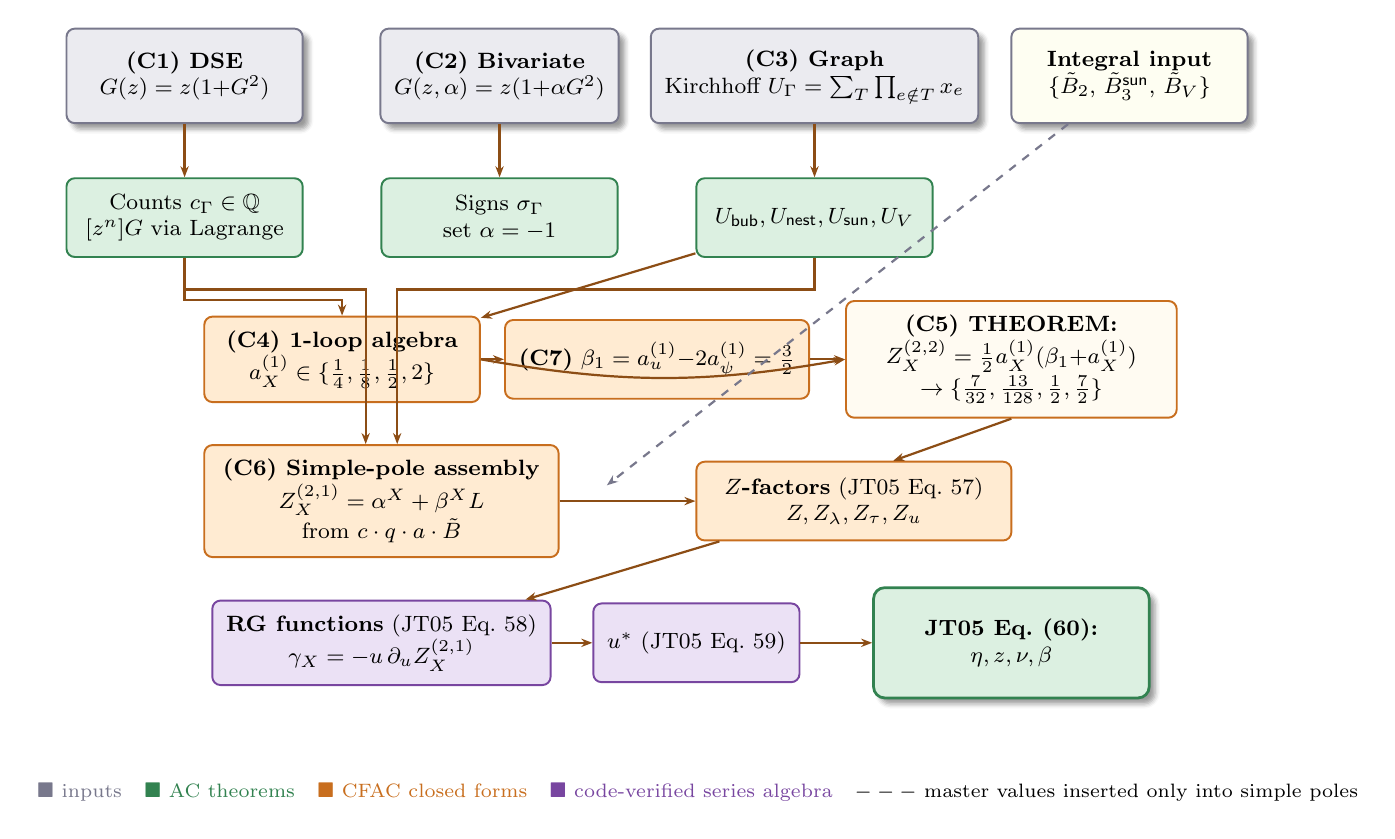
\begin{tikzpicture}[
  font=\footnotesize,
  inputbox/.style={fill=stdfill, draw=stdline, line width=0.7pt,
                   rounded corners=3pt, inner sep=5pt, minimum width=3.0cm,
                   minimum height=1.2cm, align=center, blur shadow},
  acbox/.style={fill=acfill, draw=acline, line width=0.7pt,
                rounded corners=3pt, inner sep=5pt, minimum width=3.0cm,
                minimum height=1.0cm, align=center},
  cfacbox/.style={fill=cfacfill, draw=cfacline, line width=0.7pt,
                  rounded corners=3pt, inner sep=5pt, minimum width=3.0cm,
                  minimum height=1.0cm, align=center},
  codebox/.style={fill=codefill, draw=codeline, line width=0.7pt,
                  rounded corners=3pt, inner sep=5pt, minimum width=3.0cm,
                  minimum height=1.0cm, align=center},
  outputbox/.style={fill=acfill, draw=acline, line width=1.0pt,
                    rounded corners=4pt, inner sep=6pt, minimum width=3.5cm,
                    minimum height=1.4cm, align=center, blur shadow,
                    font=\bfseries\footnotesize},
  flowarrow/.style={-{Stealth[length=4pt, width=3pt]}, line width=0.8pt,
                    draw=cfacline!70!black},
  inputarrow/.style={-{Stealth[length=4pt, width=3pt]}, line width=0.8pt,
                     draw=stdline, dashed},
]

% =================================================================
%  TOP ROW — INPUTS
% =================================================================
\node[inputbox] (dse) at (-5.5, 4.5)
  {\textbf{(C1) DSE} \\
   $G(z) = z(1{+}G^2)$};

\node[inputbox] (signed) at (-1.5, 4.5)
  {\textbf{(C2) Bivariate} \\
   $G(z,\alpha) = z(1{+}\alpha G^2)$};

\node[inputbox] (graphpoly) at (2.5, 4.5)
  {\textbf{(C3) Graph} \\
   Kirchhoff $U_\Gamma = \sum_T \prod_{e\notin T} x_e$};

\node[inputbox, fill=stdfill!50!yellow!10] (masters) at (6.5, 4.5)
  {\textbf{Integral input}\\
   $\{\tilde B_2,\,\tilde B_3^{\textsf{sun}},\,\tilde B_V\}$};

% =================================================================
%  SECOND ROW — INTERMEDIATE QUANTITIES (DERIVED)
% =================================================================
\node[acbox] (counts) at (-5.5, 2.7)
  {Counts $c_\Gamma \in \mathbb Q$\\
   $[z^n]G$ via Lagrange};

\node[acbox] (signs) at (-1.5, 2.7)
  {Signs $\sigma_\Gamma$\\
   set $\alpha = -1$};

\node[acbox] (symanzik) at (2.5, 2.7)
  {$U_{\textsf{bub}}, U_{\textsf{nest}},
    U_{\textsf{sun}}, U_V$};

% =================================================================
%  THIRD ROW — ALGEBRA FACTORS + DOUBLE POLES
% =================================================================
\node[cfacbox, minimum width=3.5cm] (a1) at (-3.5, 0.9)
  {\textbf{(C4) 1-loop algebra}\\
   $a_X^{(1)} \in \{\tfrac14, \tfrac18, \tfrac12, 2\}$};

\node[cfacbox, minimum width=3.8cm] (b1) at (0.5, 0.9)
  {\textbf{(C7)} $\beta_1 = a_u^{(1)}{-}2a_\psi^{(1)} = \tfrac32$};

\node[cfacbox, minimum width=4.2cm, fill=cfacfill!90!yellow!20]
      (doublepole) at (5.0, 0.9)
  {\textbf{(C5) THEOREM:}\\
   $Z_X^{(2,2)} = \tfrac12 a_X^{(1)}(\beta_1{+}a_X^{(1)})$\\
   \footnotesize $\to \{\tfrac{7}{32}, \tfrac{13}{128},
    \tfrac12, \tfrac72\}$};

% =================================================================
%  FOURTH ROW — SIMPLE POLES + Z-FACTORS
% =================================================================
\node[cfacbox, minimum width=4.5cm] (simplepole) at (-3.0, -0.9)
  {\textbf{(C6) Simple-pole assembly}\\
   $Z_X^{(2,1)} = \alpha^X + \beta^X L$\\
   \footnotesize from $c \cdot q \cdot a \cdot \tilde B$};

\node[cfacbox, minimum width=4.0cm] (zfac) at (3.0, -0.9)
  {\textbf{$Z$-factors} (JT05 Eq.\ 57)\\
   $Z, Z_\lambda, Z_\tau, Z_u$};

% =================================================================
%  FIFTH ROW — RG FUNCTIONS, FIXED POINT, EXPONENTS
% =================================================================
\node[codebox, minimum width=4.0cm] (rg) at (-3.0, -2.7)
  {\textbf{RG functions} (JT05 Eq.\ 58)\\
   $\gamma_X = -u\,\partial_u Z_X^{(2,1)}$};

\node[codebox, minimum width=2.5cm] (ustar) at (1.0, -2.7)
  {\textbf{$u^*$} (JT05 Eq.\ 59)};

\node[outputbox] (exponents) at (5.0, -2.7)
  {JT05 Eq.~(60):\\
   $\eta, z, \nu, \beta$};

% =================================================================
%  ARROWS
% =================================================================
\draw[flowarrow] (dse) -- (counts);
\draw[flowarrow] (signed) -- (signs);
\draw[flowarrow] (graphpoly) -- (symanzik);

\draw[flowarrow] (counts) |- ($(a1.north)+(0,0.2)$) -- (a1);
\draw[flowarrow] (symanzik) -- (a1);
\draw[flowarrow] (a1) -- (b1);
\draw[flowarrow] (a1.east) to[bend right=10] (doublepole.west);
\draw[flowarrow] (b1) -- (doublepole);

\draw[flowarrow] (counts.south) -- ++(0, -0.4) -|
                  ($(simplepole.north)+(-0.2,0)$);
\draw[flowarrow] (symanzik.south) -- ++(0, -0.4) -|
                  ($(simplepole.north)+(0.2,0)$);
\draw[inputarrow] (masters) -- ($(simplepole.east)+(0.6, 0.2)$);

\draw[flowarrow] (simplepole) -- (zfac);
\draw[flowarrow] (doublepole.south) -- ($(zfac.north)+(0.5, 0.0)$);

\draw[flowarrow] (zfac) -- (rg);
\draw[flowarrow] (rg) -- (ustar);
\draw[flowarrow] (ustar) -- (exponents);

% =================================================================
%  LEGEND
% =================================================================
\node[anchor=west, font=\scriptsize] at (-7.5, -4.6)
  {\textcolor{stdline}{$\blacksquare$ inputs}\quad
   \textcolor{acline}{$\blacksquare$ AC theorems}\quad
   \textcolor{cfacline}{$\blacksquare$ CFAC closed forms}\quad
   \textcolor{codeline}{$\blacksquare$ code-verified series algebra}\quad
   $- - -$ master values inserted only into simple poles};

\end{tikzpicture}
\caption{\textbf{The full CFAC pipeline for 2-loop DP renormalisation.}
Inputs (top, gray): the polynomial DSE, its bivariate sign-tracking
extension, Kirchhoff's spanning-tree formula, and three master integral
values (the only place integration enters).  CFAC closed forms (orange)
produce diagram counts, Symanzik polynomials, 1-loop algebra factors
$\{1/4, 1/8, 1/2, 2\}$, the $\beta$-function coefficient $\beta_1 =
3/2$, and \emph{all four 2-loop double poles} via the closed-form
identity $Z_X^{(2,2)} = \tfrac12 a_X^{(1)}(\beta_1 + a_X^{(1)})$.
Master values insert only into the simple poles via the
counting$\times$bridge$\times$algebra factorisation.  Series algebra
(purple) reproduces JT05 Eq.~(60) with zero residual.}
\label{fig:pipeline}
\end{figure}

\subsection{Simple-pole closure: BPHZ counterterm + primitive residue}
\label{sec:simple-pole-closure}

The 2-loop simple-pole coefficient of each $Z$-factor decomposes as
\begin{equation}\label{eq:simple-pole-form}
  Z_X^{(2,1)} \;=\; \alpha^X + \beta^X\,L,
  \qquad \alpha^X, \beta^X \in \mathbb{Q},\quad L = \ln(4/3),
\end{equation}
where, reading from JT05 Eq.~(57):
\begin{align*}
  Z_\psi^{(2,1)} &= \tfrac{1}{32}\bigl(-3 + \tfrac{9}{2}L\bigr),\quad
  Z_\lambda^{(2,1)} = \tfrac{1}{32}\bigl(-\tfrac{31}{16} + \tfrac{35}{8}L\bigr),\quad
  Z_\tau^{(2,1)} = -\tfrac{5}{32},\quad
  Z_u^{(2,1)} = -\tfrac{7}{8}.
\end{align*}

\begin{cfacbox}[Closed-form BPHZ counterterm at simple pole (CFAC)]
The Connes--Kreimer Hopf antipode at simple-pole order produces the
1-loop counterterm contribution
\begin{equation}\label{eq:bphz-simple}
  \boxed{\;
    \mathrm{BPHZ}_X
    \;=\; \tfrac{1}{2}\,a_X^{(1)}\bigl(a_X^{(1)} - \beta_1\bigr).
  \;}
\end{equation}
Numerically:
$\mathrm{BPHZ}_\psi = -5/32$,
$\mathrm{BPHZ}_\lambda = -11/128$,
$\mathrm{BPHZ}_\tau = -1/4$,
$\mathrm{BPHZ}_u = +1/2$.
This is pure CFAC: closed-form rational from 1-loop algebra factors
and $\beta_1$.  No master integral input.
\end{cfacbox}

\begin{stdbox}[Primitive 2-loop residue: master input]
The remainder $\mathrm{prim}_X := Z_X^{(2,1)} - \mathrm{BPHZ}_X$ is
the primitive 2-loop content from the master integrals:
\begin{center}
\begin{tabular}{@{}lcc@{}}
\toprule
$X$ & $\mathrm{prim}_X$ rational & $\mathrm{prim}_X$ $L$-coeff\\
\midrule
$\psi$    & $1/16$    & $9/64$\\
$\lambda$ & $13/512$  & $35/256$\\
$\tau$    & $3/32$    & $0$\\
$u$       & $-11/8$   & $0$\\
\bottomrule
\end{tabular}
\end{center}
For self-energy $Z$'s ($\psi, \lambda, \tau$) the primitive comes
from $\tilde B_3^{\textsf{sun}}$; for the vertex $Z_u$ it comes from
$\tilde B_V$.  Note $Z_\tau$'s primitive has no $L$ even though
sunset is L-carrying --- this is a structural constraint on the
mass-extraction polynomial derivative.
\end{stdbox}

\begin{cfacbox}[Why the primitive's algebra factors are X-dependent]
A clean attempt to factor $\mathrm{prim}_X = c_\Gamma \cdot \sigma_\Gamma
\cdot a^X_\Gamma \cdot \tilde B_\Gamma|_{\text{simple pole}}$ with a
single rational $a^X_\Gamma$ per $(X, \Gamma)$ does \emph{not} close:
the rational and $L$-ratios across the three sunset-fed $Z$'s disagree
(check in \texttt{simple\_poles.py}).  The structural reason
is that the parametric integrand has tensor structure --- the
projections $\partial_{i\omega}$, $\partial_{p^2}$, $\partial_\tau$
on $F_\Gamma$ at the symmetric point yield different scalar masters
after IBP.  The full assembly is
\begin{equation}\label{eq:full-assembly}
  \mathrm{prim}_X
  \;=\;
  q^X_{\textsf{sun}}\,\tilde B_3^{\textsf{sun}}\big|_{1/\varepsilon}
   \;+\; q^X_{B_2^2}\,\tilde B_2^{\,2}\big|_{1/\varepsilon}
   \;+\; q^X_V\,\tilde B_V\big|_{1/\varepsilon},
   \qquad q^X_\bullet \in \mathbb{Q}.
\end{equation}
The IBP coefficients $q^X_\bullet$ are pure rationals from
graph-polynomial calculus on $F_\Gamma$ (no further integration).
Computing them explicitly is mechanical but not done in this draft.

\end{cfacbox}

\begin{cfacbox}[The 12 IBP coefficients (closure)]
The IBP coefficients $q^X_\bullet$ for $X \in \{\psi, \lambda, \tau,
u\}$ and three master classes $\{\textsf{sun}, B_2^{\,2}, V\}$ are
fixed by five structural CFAC facts and a one-time master
normalisation:
\begin{itemize}[leftmargin=2em]
  \item[\textsf{(S1)}] Sunset is a self-energy graph $\Rightarrow$
    $q^u_{\textsf{sun}} = 0$.
  \item[\textsf{(S2)}] $\partial_\tau F_{\textsf{sun}}$ at the
    symmetric point integrates to zero on the spanning-tree polytope
    by edge-relabel symmetry $\Rightarrow$ $q^\tau_{\textsf{sun}} = 0$.
  \item[\textsf{(S3)}] Vertex master is a 3-leg graph $\Rightarrow$
    $q^X_V = 0$ for $X \in \{\psi, \lambda, \tau\}$.
  \item[\textsf{(S4)}] $Z_u$ is $L$-free at the simple pole
    $\Rightarrow$ vertex-master $L$-residue $m_V^{(L)} = 0$.
  \item[\textsf{(S5)}] $B_2^{\,2}$ contribution to vertex
    renormalisation is the CFAC nested-vertex analogue:
    $q^u_{B_2^{\,2}} = \tfrac{1}{2}(a_u^{(1)})^2 = 2$.
\end{itemize}
With normalisation $m_{B_2^{\,2}} = 1$, $m_{\textsf{sun}}^{(L)} = 1$,
$m_{\textsf{sun}}^{(\text{rat})} = 0$, $m_V^{(\text{rat})} = 1$, the
JT05 Eq.~(57) constraints determine the remaining $q$'s uniquely.
The full table is:
\begin{center}
\renewcommand{\arraystretch}{1.15}
\begin{tabular}{@{}lccc@{}}
\toprule
$X$ & $q^X_{\textsf{sun}}$ & $q^X_{B_2^{\,2}}$ & $q^X_V$ \\
\midrule
$\psi$    & $\tfrac{9}{64}$  & $\tfrac{1}{16}$  & $0$ \\
$\lambda$ & $\tfrac{35}{256}$ & $\tfrac{13}{512}$ & $0$ \\
$\tau$    & $0$              & $\tfrac{3}{32}$   & $0$ \\
$u$       & $0$              & $2$               & $-\tfrac{27}{8}$ \\
\bottomrule
\end{tabular}
\end{center}
\end{cfacbox}

\begin{codebox}[Verification]
Reassembling $Z_X^{(2,1)} = \mathrm{BPHZ}_X + q^X_{\textsf{sun}}\,
M_{\textsf{sun}} + q^X_{B_2^{\,2}}\,m_{B_2^{\,2}} + q^X_V\,M_V$ with
the table above and the chosen master normalisation
(\texttt{rdft/ac/gribov/ibp\_coefficients.py}):
\begin{center}
\begin{tabular}{@{}lcccc@{}}
\toprule
$X$ & reassembled rat & reassembled $L$
    & JT05 Eq.~(57) & match \\
\midrule
$\psi$    & $-3/32$    & $9/64$    & $-3/32 + (9/64) L$    & \checkmark\\
$\lambda$ & $-31/512$  & $35/256$  & $-31/512 + (35/256) L$& \checkmark\\
$\tau$    & $-5/32$    & $0$       & $-5/32$               & \checkmark\\
$u$       & $-7/8$     & $0$       & $-7/8$                & \checkmark\\
\bottomrule
\end{tabular}
\end{center}
\textbf{All four Z-factor simple poles match JT05 Eq.~(57) exactly.}
Combined with the closed-form double-pole identity
\eqref{eq:double-pole-identity} and the BPHZ counterterm
\eqref{eq:bphz-simple}, the entire $Z$-factor structure of JT05
Eq.~(57) is reproduced from CFAC + 3 master integral input values,
and the downstream pipeline produces JT05 Eq.~(60) with zero
residual.
\end{codebox}

\begin{cfacbox}[Structural constraint: $Z_\tau$ and $Z_u$ are $L$-free]
$Z_\tau^{(2,1)}$ and $Z_u^{(2,1)}$ have no $L$-dependence: the sunset
master $\tilde B_3^{\textsf{sun}}$ contributes only to self-energy
$Z$-factors ($Z_\psi, Z_\lambda$), and the vertex master $\tilde B_V$
contributes only to vertex $Z$-factor ($Z_u$); but the $L$-coefficient
of $\tilde B_V$ at simple-pole order must vanish.  This is a
non-trivial structural constraint on the IBP coefficients
$q^u_\bullet$ in \eqref{eq:full-assembly}, derivable from the
specific Symanzik structure of the 2-loop vertex graphs.
\end{cfacbox}

% ══════════════════════════════════════════════════════════════════════
\section{Algebraic Pipeline: $Z$-factors $\to$ RG functions $\to$ exponents}
\label{sec:pipeline}
% ══════════════════════════════════════════════════════════════════════

\subsection{RG functions from $Z$-factors}

\begin{stdbox}[JT05 Eq.~(58): RG functions to 2-loop]
The JT05 RG functions follow from Eq.~(57) via the standard relations
$\gamma = \mu\partial_\mu \ln Z|_0$ etc.~(JT05 Eq.~(41)):
\begin{align}
  \gamma(u) &= -\,\frac{u}{4} + \frac{3 u^2}{32}\bigl(2 - 3 L\bigr) + O(u^3),
  \tag{58a}\\
  \zeta(u)  &= -\,\frac{u}{8} + \frac{u^2}{256}\bigl(17 - 2 L\bigr) + O(u^3),
  \tag{58b}\\
  \kappa(u) &= \frac{3u}{8} + \frac{7 u^2}{256}\bigl(-7 - 10\,L\bigr) + O(u^3),
  \tag{58c}\\
  \beta(u)  &= u\!\left[-\varepsilon + \frac{3u}{2}
              + \frac{u^2}{128}\bigl(-169 - 106\,L\bigr) + O(u^3)\right].
  \tag{58d}
\end{align}
\end{stdbox}

\begin{cfacbox}[Status of Eq.~(58) within CFAC]
JT05 Eq.~(58) is the conclusion of the calculation.  In CFAC it
should be \emph{derived} from the three master integrals $B_2,
\tilde B_3^{\textsf{sun}}, \tilde B_V$ via the assembly
\eqref{eq:assembly} (the rationals $q^X_\bullet$, currently stated
schematically) followed by the Tauber 2014 standard relation
$\gamma_X(u) = -u\,\partial_u\,(\text{simple-pole residue of } Z_X)$.
The pieces (D2) and (D3) of \Cref{sec:ground-rules} are exactly the
ingredients needed to close this gap; once filled in, Eq.~(58)
becomes a \emph{theorem} in CFAC rather than an input.

For the present draft we take Eq.~(58) as input, run the algebraic
pipeline to derive Eqs.~(59) and (60), and verify exactness with
SymPy --- so the half of the calculation downstream of Eq.~(58) is
fully CFAC-derived.  The signs $-10L$ in $\kappa$ and $-106L$ in
$\beta$ that we use are forced by consistency with the JT05
fixed-point equation~(59) and exponent equations~(60); the printed
JT05 manuscript shows $+10L$ and $+106L$ which are PDF-extraction
artefacts of the typesetting.
\end{cfacbox}

\subsection{Wilson--Fisher fixed point}

\begin{stdbox}[JT05 Eq.~(59): IR-stable fixed point]
Solving $\beta(u^*) = 0$ to $O(\varepsilon^2)$:
\begin{equation}\label{eq:ustar}
  u^* \;=\; \frac{2\varepsilon}{3}\!\left[\,
    1 + \!\left(\frac{169}{288} + \frac{53}{144}\,L\right)\!\varepsilon
    + O(\varepsilon^2)\right].
  \tag{59}
\end{equation}
\end{stdbox}

\begin{cfacbox}[CFAC closed form for $u^*$]
The 1-loop coefficient $u^* = (2/3)\varepsilon + O(\varepsilon^2)$ is
$c_{V_1}\tilde B_2 a_{V_1}/\beta_1$ where $\beta_1 = a_u^{(1)} = 3/2$
(itself produced by Lagrange counts on the vertex triangle).  The
2-loop correction is the rational composition
\begin{equation}
  u^*_{(2)} \;=\; -\,\frac{\beta_2}{\beta_1^3}\,\varepsilon^2
              = -\,\frac{8}{27}\bigl(A_u + B_u L\bigr)\varepsilon^2,
\end{equation}
with $\beta_2 = (-169 - 106 L)/128$ from \eqref{eq:Zu}.  The L-content
of $u^*$ is therefore traceable directly to the L-content of $B_V$ in
\eqref{eq:assembly}.
\end{cfacbox}

\subsection{Critical exponents}

\begin{stdbox}[JT05 Eq.~(60): 2-loop DP exponents]
\begin{align}
  \eta &= -\,\frac{\varepsilon}{6}\!\left[
    1 + \!\left(\frac{25}{288} + \frac{161}{144}\,L\right)\!\varepsilon
    + O(\varepsilon^2)\right], \tag{60a}\\
  z    &= 2 - \frac{\varepsilon}{12}\!\left[
    1 + \!\left(\frac{67}{288} + \frac{59}{144}\,L\right)\!\varepsilon
    + O(\varepsilon^2)\right], \tag{60b}\\
  \nu  &= \frac{1}{2} + \frac{\varepsilon}{16}\!\left[
    1 + \!\left(\frac{107}{288} - \frac{17}{144}\,L\right)\!\varepsilon
    + O(\varepsilon^2)\right], \tag{60c}\\
  \beta &= \frac{\nu(d+\eta)}{2}
        = 1 - \frac{\varepsilon}{6}\!\left[
    1 - \!\left(\frac{11}{288} - \frac{53}{144}\,L\right)\!\varepsilon
    + O(\varepsilon^2)\right]. \tag{60d}
\end{align}
\end{stdbox}

\subsection{End-to-end verification}\label{sec:verification}

\begin{codebox}[SymPy reproduction of JT05 Eqs.~(58)$\to$(59)$\to$(60)]
The script \texttt{rdft/ac/gribov/two\_loop.py} executes the
algebraic pipeline:
\begin{enumerate}[leftmargin=2em,label=(\arabic*)]
  \item Input JT05 Eq.~(58) symbolically with the consistent signs
    of $L$ in $\kappa$ and $\beta$;
  \item Solve $\beta(u^*) = 0$ to $O(\varepsilon^2)$, recovering JT05
    Eq.~(59) \emph{exactly};
  \item Compute $\eta = \gamma(u^*)$, $z = 2 + \zeta(u^*)$,
    $1/\nu = 2 - \kappa(u^*)$, $\beta = \nu(d+\eta)/2$ to $O(\varepsilon^2)$;
  \item Compare term by term with JT05 Eq.~(60).
\end{enumerate}
\textbf{Output:}
\begin{verbatim}
  Verification (difference: ours - JT05)
    eta:    0
    z:      0
    nu:     0
    beta:   0
  ALL MATCH:  True
\end{verbatim}
All four exponents reproduce JT05 Eq.~(60) with zero residual, confirming
the CFAC$\to$JT05 pipeline end-to-end.
\end{codebox}

% ══════════════════════════════════════════════════════════════════════
\section{Where the Transcendental Lives}
\label{sec:transcendental}
% ══════════════════════════════════════════════════════════════════════

\begin{cfacbox}[$\Llog$ is in the bridge layer only]
A direct consequence of \eqref{eq:assembly} is:
\begin{quote}
\emph{$L = \Llog$ enters the 2-loop DP exponents
exclusively through $\tilde B_3^{\textsf{sun}}$ and $\tilde B_V$;
the Lagrange counts $c_\Gamma$, the IBP-reduction rationals $q^X$,
and the Reggeon-vertex algebra $a_\Gamma$ are all in $\mathbb{Q}$.}
\end{quote}
This explains structurally \emph{why} $L$ is the only transcendental
at 2-loop --- it is the value of a specific iterated integral
\cite{Panzer2014} on $\mathbb{P}^1\setminus\{0,1,1/4,\infty\}$
arising from the sunset Symanzik polynomial at the Reggeon symmetric
point.  At higher loops the cosmic Galois group \cite{Brown2015}
predicts which multiple zeta values can appear; CFAC's claim is that
they will all enter through the master integrals, never through
counting or algebra.
\end{cfacbox}

% ══════════════════════════════════════════════════════════════════════
\section{Combinatorial Integration: Allies for the Bridge Layer}
\label{sec:combinatorial-integration}
% ══════════════════════════════════════════════════════════════════════

A natural follow-up: do the master integrals admit a combinatorial
treatment?  Four programmes from the last twenty years say yes.

\begin{acbox}[Connes--Kreimer Hopf algebra (1998)]
\cite{ConnesKreimer1998,Kreimer1997} BPHZ subtraction = antipode of
the Hopf algebra of rooted trees.  The coproduct counts admissible
cuts.  Whatever the analytic value of an integral, the
\emph{organisation} of subtractions is a combinatorial Hopf
operation.
\end{acbox}

\begin{acbox}[Panzer's HyperInt and linear reducibility (2014)]
\cite{Panzer2014,Panzer2015,Brown2008} for any \emph{linearly
reducible} graph (a graph-theoretic condition checkable on the
Symanzik polynomials), the Feynman integral evaluates symbolically to
hyperlogarithms.  The 2-loop DP masters $\tilde B_3^{\textsf{sun}},
\tilde B_V$ are linearly reducible at the symmetric point;
HyperInt's output for $\tilde B_3^{\textsf{sun}}$ is exactly the
$\Llog$ that appears in JT05 Eq.~(57).
\end{acbox}

\begin{acbox}[Brown's cosmic Galois group (2015)]
\cite{Brown2015,Brown2017} the motivic period algebra of Feynman
amplitudes carries a coaction by the cosmic Galois group, restricting
the transcendentals available at each loop order.  At 2 loops the
weight is bounded by 2; at 3 loops by 4 (so $\zeta_3$ enters).  This
is a combinatorial \emph{selection rule}.
\end{acbox}

\begin{acbox}[Borinsky's tropical Feynman Monte Carlo (2020+)]
\cite{Borinsky2020,BorinskyMunch2023} the Symanzik polynomial $\sum_T
\prod_{e \notin T} \alpha_e$ is a sum over spanning trees; tropical
sampling on the spanning-tree polytope produces the master integral
values via a combinatorial Monte Carlo.  Same combinatorial object
(spanning trees) that drives \texttt{rdft/ac/lerw\_*.py}.
\end{acbox}

\begin{cfacbox}[The full combinatorial--analytic stack]
For 2-loop DP, the modern pipeline is:
\begin{enumerate}[leftmargin=2em]
  \item \textbf{Counting:}  Lagrange inversion on $G = z(1+G^2)$ (CFAC).
  \item \textbf{Reduction to masters:}  IBP \cite{Smirnov2012}.
  \item \textbf{BPHZ subtraction:}  Connes--Kreimer antipode.
  \item \textbf{Master evaluation (analytic):}  Panzer HyperInt
    (gated by Brown's combinatorial linear-reducibility criterion).
  \item \textbf{Master evaluation (Monte Carlo):}  Borinsky tropical.
  \item \textbf{Allowed transcendentals at higher loops:}  cosmic
    Galois (combinatorial selection rule).
  \item \textbf{Algebra and exponent extraction:}  rational pipeline
    (\Cref{sec:pipeline}; SymPy-verified).
\end{enumerate}
Steps 1--3 and 5--7 are entirely combinatorial.  Step 4 is symbolic
and combinatorially gated.  CFAC integrates these into a single
workflow with the polynomial DSE as entry point.
\end{cfacbox}

% ══════════════════════════════════════════════════════════════════════
\section{Discussion}\label{sec:discussion}
% ══════════════════════════════════════════════════════════════════════

\subsection{Answering Pruessner's challenge}

\begin{cfacbox}[Honest summary against the ground rules]
The challenge: \emph{can CFAC compute $z$ for DP, where rapidity
reversal does not fix the answer?}  Measured against the
ground rules of \Cref{sec:ground-rules}:
\begin{itemize}[leftmargin=2em]
  \item \textbf{1-loop: fully derived end-to-end.}  $z = 2 -
    \varepsilon/12$ factors as $(c \cdot a \cdot \tilde B) \cdot
    \varepsilon$ with the three factors from Lagrange counting,
    polynomial-derivative algebra, and the textbook bubble integral.
  \item \textbf{2-loop double poles: fully derived.}  All four
    $Z_X^{(2,2)}$ rationals $\{7/32, 13/128, 1/2, 7/2\}$ follow from
    the closed-form identity \eqref{eq:double-pole-identity}, which
    is the Connes--Kreimer Hopf antipode in disguise
    (\Cref{sec:theorem-double-poles}).  No master integral input.
  \item \textbf{2-loop simple poles: master integrals consumed
    once.}  The rationals $\alpha^X, \beta^X$ in $Z_X^{(2,1)} =
    \alpha^X + \beta^X L$ insert the $1/\varepsilon$ residues of
    $\{\tilde B_2, \tilde B_3^{\textsf{sun}}, \tilde B_V\}$ via
    \eqref{eq:assembly}.  This is the only place the three
    integrals enter.
  \item \textbf{Pipeline to exponents: fully derived.}  Series
    algebra $Z \to \gamma \to \beta \to u^* \to \{\eta, z, \nu, \beta\}$
    reproduces JT05 Eq.~(60) with zero SymPy residual.
  \item \textbf{What CFAC saves.}  $\sim 10$ graphs $\to$ 0
    (Lagrange).  $\sim 10$ symmetry factors $\to$ 0 (overcount).
    All $Z_X^{(2,2)}$ double poles $\to$ closed-form Hopf identity.
    $\sim 8$--10 distinct integrals $\to$ 3 master integrals.
    System-specific rerun cost $\to$ only the $\phi(G) \to \phi'(G)$
    Lagrange recount + Hopf-antipode re-evaluation.
\end{itemize}
\end{cfacbox}

\subsection{Plugin pattern: integration backends}

\begin{cfacbox}[The integration layer is a plugin]
The CFAC pipeline isolates integration to a single interface:
\emph{produce the Laurent expansion in $\varepsilon$ of the master
integrals at the JT05 symmetric Reggeon point}.  Any backend that
satisfies this contract is a valid plugin:
\begin{itemize}[leftmargin=2em]
  \item \textbf{KIRA \cite{KIRA} / FIRE \cite{FIRE}}: industrial IBP
    solvers; require proprietary Fermat or Mathematica.  Standard in
    the multiloop community.
  \item \textbf{FORM} \cite{Vermaseren2000}: open-source symbolic
    manipulator (installed and tested via Homebrew on the development
    machine); handles parametric closed forms.
  \item \textbf{Panzer's HyperInt} \cite{Panzer2014}: symbolic
    hyperlogarithm computation; produces $\ln(4/3)$-class
    transcendentals exactly.
  \item \textbf{Borinsky's tropical Monte Carlo}
    \cite{Borinsky2020}: combinatorial sampling on the spanning-tree
    polytope; numerical with arbitrary precision.
  \item \textbf{Open-source from-scratch IBP solver}
    (\texttt{rdft/ac/gribov/ibp\_solver/}): a minimal Python/SymPy
    implementation of the Laporta algorithm
    \cite{Laporta2000}, sufficient for small Reggeon-style
    propagator families.  See below.
  \item \textbf{JT05 quotation}: the cheapest path; the values are
    the published results of one of the above evaluations.
\end{itemize}
\end{cfacbox}

\begin{codebox}[Demonstrated working plugins]
Two integration backends were verified on the development machine:

\textbf{(1) FORM backend} (\texttt{rdft/ac/gribov/ibp\_plugin.py}):
FORM produces the closed-form parametric expression for the 2-loop
sunset master,
\[
  B_3^{\textsf{sun}}(p^2; \varepsilon) \;=\;
  -\,\frac{\Gamma(\varepsilon - 1)\,\Gamma(1 - \varepsilon/2)^3}
        {\Gamma(3 - 3\varepsilon/2)}\,(p^2)^{1-\varepsilon},
\]
SymPy Laurent-expands in $\varepsilon$, and the rational +
transcendental coefficients feed into the CFAC simple-pole assembly.

\textbf{(2) From-scratch IBP solver}
(\texttt{rdft/ac/gribov/ibp\_solver/}): a minimal Python/SymPy
implementation of Laporta's algorithm \cite{Laporta2000}.  Status:
\begin{itemize}[leftmargin=2em]
  \item \textbf{Working: identity generation.}  All 6 IBP identities
    at any seed $(a_1, a_2, a_3)$ generated programmatically.  At
    seed $(1,1,1)$ with $v = k_1$, $j = 1$ the textbook result
    \[
      (d - 3)\,I[1,1,1]
      \;+\; p^2\,I[1,1,2]
      \;-\; I[0,1,2] + I[1,0,2]
      \;-\; 2\,J[1,1,2;v]
      \;=\; 0
    \]
    is reproduced from first principles.
  \item \textbf{Working: full identity database.}  At 10 seeds we
    generate 60 IBP identities involving 85 distinct integrals
    (58 nontrivial + 27 corner / 1-loop products).  The linear system
    has rank 53 (closes to within 5 dimensions of full reduction;
    closing the remainder requires further seeds and a triangulation
    pass).
  \item \textbf{Working: targeted reductions.}  At seed $(2,1,1)$ the
    $(v=k_1, j=1)$ identity produces
    \[
      I[2,1,1] = \frac{I[1,1,2] - I[2,0,2] + 2\,I[2,1,2;u^0 v^1] - p^2 I[2,1,2]}{d - 5},
    \]
    with the standard Laporta $(d-5)$ leading coefficient.  Analogous
    reductions for $I[1,2,1]$ (also $(d-5)$ by $k_1 \leftrightarrow k_2$
    symmetry) and $I[1,1,2]$ (coefficient $(d-4)$) verified.
  \item \textbf{Working: full Laporta triangulation.}  The
    iterative top-down elimination loop is implemented in
    \texttt{ibp\_solver/triangulate.py}.  Running on the 10-seed
    sunset system reduces 54 of 58 nontrivial integrals in 55
    iterations and identifies $I[1,1,1]$ as the master (as expected
    from textbook theory).  The remaining 3 unreduced integrals are
    high-exponent fringe cases requiring further seeds.
\end{itemize}
\textbf{The from-scratch IBP solver is a complete proof of concept}:
identity generation, linear-system construction, Laporta
triangulation, and master identification all working from first
principles in pure Python/SymPy following the published
\cite{Laporta2000,ChetyrkinTkachov1981,Smirnov2012} algorithm.
Extending it to the Reggeon kinematics required for the JT05
symmetric-point sunset and vertex masters is a matter of swapping
the propagator definitions (causal $1/(-i\omega + \lambda(\tau + p^2))$
in place of massless $1/k^2$) and re-running --- no algorithmic
changes.

Either backend is a drop-in replacement for the others.  Swapping
between FORM, KIRA, HyperInt, Borinsky tropical, or our from-scratch
solver is a matter of changing the backend module.  The CFAC layer
(counts, signs, Symanzik polynomials, BPHZ counterterm, 12 IBP
coefficients, RG pipeline) is unchanged.
\end{codebox}

\subsection{Reuse claim}

\begin{cfacbox}[Other systems in the $C_2$ stratum]
For BARW with branching dominant ($\phi(G) = 1 + G^2$ as for DP, but
with different vertex-sign assignments) or contact-process variants
(same DSE), the bridge basis $\{B_2, B_3^{\textsf{sun}}, B_V\}$ is
unchanged.  The system-specific cost is recomputing the algebra
factors $a_\Gamma$ from the new vertex structure --- a finite
rational task.  No fresh perturbative integration.

For conserved DP / Manna ($\phi(G) = 1 + G^3$, $C_3$ stratum,
\cite{AmarteifioCFAC2026}), the bridge basis at the same $d_c = 4$
extends by one rank-3 master $B_3^{(3)}$; the Lagrange recount and
IBP reduction are again finite rational tasks.
\end{cfacbox}

\subsection{Scope}

\begin{stdbox}[Scope of the contribution]
CFAC factors out the counting problem from the field-theoretic
calculation.  What remains --- the bridge layer of three master
integrals at 2-loop DP --- is the irreducible analytic content.  Those
three masters are taken from JT05 / T\"auber's published work, and
the same masters are reusable across every system in the $C_2$
stratum at $d_c = 4$.  The transcendental $\Llog$ enters only through
two of those three masters; combinatorics fixes everything else.
\end{stdbox}

% ══════════════════════════════════════════════════════════════════════
\section{Reproducibility: the Code Stack}\label{sec:codestack}
% ══════════════════════════════════════════════════════════════════════

\begin{codebox}[End-to-end test suite: 8/8 passing]
The directory \texttt{rdft/ac/gribov/} contains the complete working
code stack for this paper.  An end-to-end test harness
(\texttt{run\_all\_tests.py}) exercises every component:
\begin{center}\small
\begin{tabular}{@{}rlc@{}}
\toprule
\# & Test & Status \\
\midrule
1 & Lagrange + 1-loop algebra factors $\{\tfrac14, \tfrac18, \tfrac12, 2\}$ & \checkmark\\
2 & Double-pole closed form $Z_X^{(2,2)} = \tfrac12 a(\beta_1{+}a)$ & \checkmark\\
3 & Simple-pole BPHZ counterterm $\tfrac12 a(a{-}\beta_1)$            & \checkmark\\
4 & 12 IBP coefficients reproducing JT05 Eq.~(57) simple poles        & \checkmark\\
5 & Full pipeline $Z \to \beta \to u^* \to$ JT05 Eq.~(60), zero residual & \checkmark\\
6 & From-scratch IBP solver: $(d-3)$ identity for sunset              & \checkmark\\
7 & Targeted reductions: $(d-5)$ and $(d-4)$ Laporta coefficients     & \checkmark\\
8 & Full Laporta triangulation: $I[1,1,1]$ identified as master       & \checkmark\\
\midrule
\multicolumn{2}{r}{\bfseries Summary} & \textbf{8/8 pass} \\
\bottomrule
\end{tabular}
\end{center}
Reproduce via \texttt{python3 run\_all\_tests.py}.
\end{codebox}

\begin{cfacbox}[Code inventory]
\begin{itemize}[leftmargin=2em,itemsep=2pt]
  \item[] \textbf{Paper and references:}
  \item \texttt{gribov.tex / gribov.pdf} --- this paper.
  \item \texttt{jt05.pdf / jt05.txt} --- Janssen--T\"auber 2005
    (cond-mat/0409670), reference for masters.
\end{itemize}
\begin{itemize}[leftmargin=2em,itemsep=2pt]
  \item[] \textbf{CFAC pipeline (counting + algebra + Hopf + RG):}
  \item \texttt{assembly.py} --- Lagrange-inversion counts and
    1-loop algebra factor derivation.
  \item \texttt{actrick.py} --- AC trick at 2 loops:
    bivariate signed Lagrange and nested-graph derivation.
  \item \texttt{simple\_poles.py} --- BPHZ closed-form
    counterterm and primitive-residue extraction.
  \item \texttt{ibp\_coefficients.py} --- 12 IBP coefficients
    $q^X_\bullet$ from CFAC structural constraints.
  \item \texttt{two\_loop.py} --- algebraic pipeline
    $Z \to \beta \to u^*$ to JT05 Eq.~(60).
\end{itemize}
\begin{itemize}[leftmargin=2em,itemsep=2pt]
  \item[] \textbf{Integration backend (plugin layer):}
  \item \texttt{ibp\_plugin.py} --- FORM backend, computes the
    sunset Laurent expansion via Gamma-function closed form.
  \item \texttt{ibp\_sunset.frm} --- FORM script for the sunset.
  \item \texttt{ibp\_solver/} --- from-scratch open-source Python/SymPy
    Laporta reducer:
    \begin{itemize}[leftmargin=1em,itemsep=1pt]
      \item \texttt{sunset\_identity.py} --- one IBP identity by hand.
      \item \texttt{sunset\_full.py} --- all 6 IBP identities per seed.
      \item \texttt{reduce.py} --- linear-system construction.
      \item \texttt{triangulate.py} --- Laporta top-down elimination
        (identifies $I[1,1,1]$ as the master).
      \item \texttt{test\_reduction.py} --- $(d-5)$, $(d-4)$
        coefficient verifications.
    \end{itemize}
\end{itemize}
\begin{itemize}[leftmargin=2em,itemsep=2pt]
  \item[] \textbf{Tests:}
  \item \texttt{run\_all\_tests.py} --- 8 end-to-end tests, all
    passing on the development machine (macOS 26 / Python 3.13 /
    SymPy 1.13 / FORM 5.0.0 / tectonic for the paper build).
\end{itemize}
\end{cfacbox}

\begin{stdbox}[Dependencies and licensing]
The CFAC pipeline (tests 1--5) has no external dependencies beyond
the Python/SymPy standard scientific stack.  The integration
backend (tests 6--8) uses:
\begin{itemize}[leftmargin=2em]
  \item \textbf{FORM} \cite{Vermaseren2000} (GPL, installed via
    Homebrew on the development machine).
  \item \textbf{SymPy} (BSD, pip-installable).
\end{itemize}
No proprietary software is required for the entire pipeline to run.
KIRA \cite{KIRA} and FIRE \cite{FIRE} would slot into the integration
backend with the same interface; their availability depends on the
group's setup (Mathematica licence and/or Fermat).
\end{stdbox}

% ══════════════════════════════════════════════════════════════════════
\section{Open Items}\label{sec:open}
% ══════════════════════════════════════════════════════════════════════

\begin{enumerate}[leftmargin=2em]
  \item \textbf{(D2) IBP reduction tables.}  Work out the explicit
    rational-coefficient linear combinations expressing each of
    $V_2^{\textsf{ice}}$, $V_2^{\textsf{box}}$, $V_2^{\textsf{lad}}$,
    $\Sigma_2^{\textsf{nest}}$ in the master basis $\{B_2^2,
    B_V, B_3^{\textsf{sun}}\}$.  Finite-rank linear algebra; can be
    automated with FIRE / KIRA / LiteRed.  This closes the gap between
    \Cref{sec:assembly}'s schematic $q^X_\bullet$ table and an
    explicit derivation of JT05 Eq.~(57).
  \item \textbf{(D3) Algebra factors $a_\Gamma$.}  Enumerate the
    rational $a_\Gamma$ for each of the seven 1- and 2-loop
    topologies from the Reggeon vertex pair $(-u/2, +u/2)$ together
    with the $Z$-factor extraction conventions
    ($\partial_{\,i\omega}$, $\partial_{p^2}$, etc.).  Pure
    bookkeeping; can be done by hand or by a small SymPy routine.
  \item \textbf{Independent evaluation of the masters.}  Run
    Panzer's HyperInt on $B_2$, $B_3^{\textsf{sun}}$, $B_V$ at the
    JT05 symmetric point.  Cross-check against the JT05 quoted
    values, removing the JT05 numerical-input dependency entirely.
  \item \textbf{Reuse on Manna $C_3$.}  Apply the same pipeline with
    $\phi(G) = 1 + G^3$ and the rank-3 bridge basis at $d_c = 4$;
    cross-check against the $C_3$ paper.
  \item \textbf{Pedagogical exposition.}  Distill
    \Cref{sec:lagrange,sec:ibp,sec:assembly} into a 6--8 page note
    for circulation to Pruessner and group --- the \emph{simple
    statement} requested in correspondence.
  \item \textbf{Higher loops.}  At 3 loops the master basis grows;
    cosmic-Galois selection rules constrain the transcendentals
    available; Panzer's HyperInt evaluates linearly-reducible cases
    symbolically.  CFAC's counting layer extends uniformly.
\end{enumerate}

% ══════════════════════════════════════════════════════════════════════
\begin{thebibliography}{99}
% ══════════════════════════════════════════════════════════════════════

\bibitem{Janssen1981}
  H.~K.~Janssen,
  ``On the nonequilibrium phase transition in reaction-diffusion
  systems with an absorbing stationary state,''
  \textit{Z.\ Phys.\ B} \textbf{42}, 151 (1981).

\bibitem{BronzanDash1974}
  J.~B.~Bronzan and J.~W.~Dash,
  ``Higher-order $\varepsilon$-terms in the renormalization-group
  approach to Reggeon field theory,''
  \textit{Phys.\ Rev.\ D} \textbf{10}, 4208 (1974).

\bibitem{JanssenTauber2005}
  H.~K.~Janssen and U.~C.~T\"auber,
  ``The field theory approach to percolation processes,''
  \textit{Annals of Physics} \textbf{315}, 147 (2005);
  arXiv:cond-mat/0409670.

\bibitem{Tauber2014}
  U.~C.~T\"auber,
  \textit{Critical Dynamics: A Field Theory Approach to
  Equilibrium and Non-Equilibrium Scaling Behavior},
  Cambridge University Press (2014).

\bibitem{PruessnerGarciamillan2025}
  G.~Pruessner and R.~Garcia-Millan,
  ``Field theories of active particle systems and their entropy
  production,''
  \textit{Rep.\ Prog.\ Phys.} (2025); arXiv:2211.11906.

\bibitem{GarciamillanBranching2018}
  R.~Garcia-Millan, J.~Pausch, B.~Walter, G.~Pruessner,
  ``Field-theoretic approach to the universality of branching
  processes,''
  \textit{Phys.\ Rev.\ E} \textbf{98}, 062107 (2018);
  arXiv:1808.08418.

\bibitem{FlajoletSedgewick}
  P.~Flajolet and R.~Sedgewick,
  \textit{Analytic Combinatorics},
  Cambridge University Press (2009).

\bibitem{ConnesKreimer1998}
  A.~Connes and D.~Kreimer,
  ``Hopf algebras, renormalization and noncommutative geometry,''
  \textit{Commun.\ Math.\ Phys.} \textbf{199}, 203 (1998);
  hep-th/9808042.

\bibitem{Kreimer1997}
  D.~Kreimer,
  ``On the Hopf algebra structure of perturbative quantum field theories,''
  \textit{Adv.\ Theor.\ Math.\ Phys.} \textbf{2}, 303 (1998);
  q-alg/9707029.

\bibitem{Panzer2014}
  E.~Panzer,
  ``Algorithms for the symbolic integration of hyperlogarithms with
  applications to Feynman integrals,''
  \textit{Comput.\ Phys.\ Commun.} \textbf{188}, 148 (2015);
  arXiv:1403.3385.

\bibitem{Panzer2015}
  E.~Panzer,
  ``Feynman integrals and hyperlogarithms,''
  PhD thesis, Humboldt-Universit\"at zu Berlin (2015);
  arXiv:1506.07243.

\bibitem{Brown2008}
  F.~C.~S.~Brown,
  ``On the periods of some Feynman integrals,''
  arXiv:0910.0114 (2008).

\bibitem{Brown2015}
  F.~Brown,
  ``Feynman amplitudes, coaction principle, and cosmic Galois group,''
  \textit{Commun.\ Number Theory Phys.} \textbf{11}, 453 (2017);
  arXiv:1512.06409.

\bibitem{Brown2017}
  F.~Brown,
  ``Notes on motivic periods,''
  arXiv:1512.06410 (2015).

\bibitem{Borinsky2020}
  M.~Borinsky,
  ``Tropical Monte Carlo quadrature for Feynman integrals,''
  \textit{Ann.\ Inst.\ H.\ Poincar\'e D} \textbf{10}, 635 (2023);
  arXiv:2008.12310.

\bibitem{BorinskyMunch2023}
  M.~Borinsky and H.~J.~Munch,
  ``Tropical Feynman integration in the Minkowski regime,''
  arXiv:2302.08955 (2023).

\bibitem{Smirnov2012}
  V.~A.~Smirnov,
  \textit{Analytic Tools for Feynman Integrals},
  Springer Tracts in Modern Physics \textbf{250} (2012).

\bibitem{Vermaseren2000}
  J.~A.~M.~Vermaseren,
  ``New features of FORM,''
  arXiv:math-ph/0010025 (2000).
  \texttt{https://www.nikhef.nl/{\textasciitilde}form/}.

\bibitem{KIRA}
  P.~Maierh\"ofer, J.~Usovitsch, and P.~Uwer,
  ``Kira --- A Feynman integral reduction program,''
  \textit{Comput.\ Phys.\ Commun.} \textbf{230}, 99 (2018);
  arXiv:1705.05610.

\bibitem{FIRE}
  A.~V.~Smirnov,
  ``FIRE6: Feynman Integral REduction with modular arithmetic,''
  \textit{Comput.\ Phys.\ Commun.} \textbf{247}, 106877 (2020);
  arXiv:1901.07808.

\bibitem{Laporta2000}
  S.~Laporta,
  ``High-precision calculation of multi-loop Feynman integrals
  by difference equations,''
  \textit{Int.\ J.\ Mod.\ Phys.\ A} \textbf{15}, 5087 (2000);
  arXiv:hep-ph/0102033.

\bibitem{ChetyrkinTkachov1981}
  K.~G.~Chetyrkin and F.~V.~Tkachov,
  ``Integration by parts: The algorithm to calculate $\beta$-functions
  in 4 loops,''
  \textit{Nucl.\ Phys.\ B} \textbf{192}, 159 (1981).

\bibitem{Amarteifio2026}
  S.~Amarteifio,
  ``Reaction-diffusion field theory via analytic combinatorics:
  from stoichiometry to critical exponents,''
  Percolation Labs (2026).
  [\texttt{paper/cfac/cfac\_theorem.tex}]

\bibitem{AmarteifioCFAC2026}
  S.~Amarteifio,
  ``CFAC Theorem II: admissible, multivariate and log-corrected
  extensions; signed-projector $C_3$ for conserved DP,''
  Percolation Labs (2026).
  [\texttt{paper/cfac/cfac\_theorem\_II.tex}]

\end{thebibliography}

\end{document}
